% CVPR 2026 Submission
\documentclass[10pt,twocolumn,letterpaper]{article}

% CVPR/ICCV style — [review] for submission, [final] for a clean local PDF
\usepackage[final]{iccv}

\def\confName{CVPR}
\def\confYear{2026}
\def\paperID{****}

\PassOptionsToPackage{table}{xcolor}
\usepackage[utf8]{inputenc}
\usepackage[T1]{fontenc}
\usepackage[breaklinks,colorlinks]{hyperref}
\usepackage{nicefrac}
\usepackage{microtype}
\usepackage{graphicx}
\usepackage{multirow}
\usepackage{tabularx}
\usepackage{xcolor}
\usepackage{colortbl}

\newcounter{algorithm}
\newenvironment{cvpralgorithm}{\begin{figure}[t]\refstepcounter{algorithm}\noindent\begin{minipage}{\linewidth}}{\end{minipage}\end{figure}}
\newcommand{\algorithmcaption}[1]{\noindent\emph{Algorithm \thealgorithm. #1}\par\vspace{2pt}}
\newcommand{\algkw}[1]{\emph{#1}}
\newcommand{\algindent}{\hspace*{1.2em}}
\newcommand{\algindenttwo}{\hspace*{2.4em}}

\title{Depth-Conditioned Pseudo-Labels for \\ Scene-Centric Unsupervised Panoptic Segmentation}

\author{Anonymous CVPR 2026 Submission \\
Paper ID \paperID}

\begin{document}
\raggedbottom

\maketitle

\begin{abstract}
Existing unsupervised scene-centric panoptic methods rely on calibrated stereo and unsupervised optical flow, foreclosing the long tail of monocular footage from phones, dashcams, and fixed cameras. We close this gap in two stages. First, we show that frozen monocular priors alone are sufficient to train a panoptic network to 32.76 PQ on Cityscapes val under the adopted CUPS-style trainer~\cite{hahn2025cups}. Second, we contribute two compact mechanisms that compose these priors through cross-modal agreement --- DCFA, a $\sim$225K-parameter residual adapter that conditions a frozen unsupervised semantic code on monocular depth; and SIMCF, a learning-free filter that enforces semantic, geometric, and appearance agreement on candidate panoptic labels --- improving this controlled monocular baseline by $+3.07$ PQ. The resulting 35.83 PQ also surpasses the published stereo+flow CUPS configuration~\cite{hahn2025cups} (27.80 PQ) under the reported CUPS evaluation protocol~\cite{hahn2025cups}, while using only single monocular target images at pseudo-label time.
\end{abstract}

\begin{figure*}[t]
\centering
\includegraphics[width=\textwidth]{../figures/paper_ready/pipeline_overview.png}
\caption{Pipeline overview. Stage 1 constructs panoptic pseudo-labels from a single RGB image using frozen semantic features, monocular depth, DCFA, and SIMCF. Stage 2 adopts CUPS-style~\cite{hahn2025cups} panoptic bootstrapping and panoptic network training on the filtered labels.}
\label{fig:pipeline_overview}
\end{figure*}


%=========================================================================
\section{Introduction}
\label{sec:intro}
%=========================================================================

Panoptic segmentation assigns a category to every pixel and a distinct identity to every countable object. The task underpins autonomous driving, robotic manipulation, and dense scene parsing, and its supervised counterpart sits at the top of every benchmark that supplies dense human masks. The obstacle is annotation cost: Cityscapes-style annotation requires a pixel-level mask for every visible instance, and the cost compounds with each new dataset and domain. The unsupervised setting asks whether a model can recover panoptic structure from raw pixels alone.

Recent progress has come from three lineages. Self-supervised semantic discovery on top of frozen DINO/DINOv2 features~\cite{caron2021dino,oquab2024dinov2} now yields region-level partitions coherent enough to serve as semantic pseudo-labels~\cite{hamilton2022stego,kim2024cause}. Cut-and-learn instance discovery~\cite{simeoni2021lost,wang2023tokencut,wang2023cutler} extracts foreground masks from the same SSL features and bootstraps detectors from them. CutS3D~\cite{sick2025cuts3d} moves this instance line toward scene-centric data by lifting depth to a 3-D point cloud and applying LocalCut to disambiguate adjacent instances. CUPS~\cite{hahn2025cups} combines semantic pseudo-labels, stereo-derived depth, and unsupervised scene flow, then trains a Cascade Mask R-CNN with DropLoss bootstrapping and EMA self-training.

CUPS~\cite{hahn2025cups} obtains this structure from calibrated stereo at pseudo-label time and unsupervised optical flow over short video clips. These inputs are not available for many scene-centric datasets, where images often arrive as single monocular frames from a phone, dashcam, or fixed camera. A method that depends on multi-view input therefore narrows the range of imagery where unsupervised panoptic segmentation can be applied. We ask whether this extra input is necessary, or whether monocular images already contain enough structure for pseudo-label generation.

We show that frozen monocular priors can replace stereo and motion at pseudo-label time when they are combined through cross-modal agreement. Semantic codes provide class-consistent regions but may merge adjacent same-class objects or split a surface under illumination change. Monocular depth provides physical separations but may over-fragment objects along material seams. Dense feature similarity can merge depth fragments when their appearance is compatible. Our pipeline uses these cues conservatively: depth proposes candidate boundaries, while semantic identity and feature similarity decide which boundaries should survive.

This design improves pseudo-label panoptic quality from 24.54 to 25.85 on Cityscapes before panoptic bootstrapping. After CUPS-style~\cite{hahn2025cups} panoptic bootstrapping and panoptic network training, the final model reaches 35.83 PQ, 62.79 SQ, and 43.78 RQ on Cityscapes val. The corresponding monocular baseline without DCFA/SIMCF reaches 32.76 PQ under the same training procedure, isolating a +3.07 PQ gain from the proposed pseudo-label generator. The published CUPS configuration~\cite{hahn2025cups} reaches 27.80 PQ with stereo + motion cues at pseudo-label time.

We make three contributions:
\begin{itemize}
\item Stereo-and-motion-free pseudo-label generation for scene-centric panoptic segmentation. Monocular semantic appearance and monocular depth, composed by an agreement filter, supply enough structure for scene-centric unsupervised panoptic-label generation, removing the stereo + motion requirement in CUPS~\cite{hahn2025cups} at pseudo-label time.
\item Two compact mechanisms for cross-modal agreement. A depth-conditioned residual adapter (DCFA) adapts a frozen 90-dimensional semantic code toward depth-consistent regions and lifts semantic mIoU from 52.69 to 55.29; Semantic Instance Mutual Consistency Filtering (SIMCF) accepts, revises, or rejects candidate labels through semantic, geometric, and appearance agreement and contributes the bulk of the +1.31 PQ pseudo-label gain.
\item 35.83 PQ on Cityscapes after panoptic network training. Using the adopted CUPS~\cite{hahn2025cups} panoptic bootstrapping and network-training procedures, the final network reaches 35.83 PQ on Cityscapes val, a +3.07 PQ gain over the corresponding monocular baseline.
\end{itemize}

Figure~\ref{fig:pipeline_overview} gives the full pipeline view. Section~\ref{sec:related} surveys the unsupervised semantic, instance, and panoptic literatures. Section~\ref{sec:method} develops the pipeline. Section~\ref{sec:experiments} reports Cityscapes results, ablations, and transfer experiments. Section~\ref{sec:discussion} discusses the results. Section~\ref{sec:limitations} summarizes the main limitations.

%=========================================================================
\section{Related Work}
\label{sec:related}
%=========================================================================

\paragraph{Unsupervised Semantic Segmentation.}
Early unsupervised semantic segmentation methods optimized clustering objectives over learned image representations: IIC~\cite{ji2019iic} maximized mutual information between augmented views, and PiCIE~\cite{cho2021picie} enforced photometric and geometric invariance to recover pixel-level groupings. The arrival of self-supervised vision transformers~\cite{caron2021dino,oquab2024dinov2} reshaped the field, with dense ViT features clustering cleanly enough that \emph{distillation} methods became dominant. STEGO~\cite{hamilton2022stego} distilled DINO correspondences into compact dense embeddings; HP~\cite{seong2023hp} improved this contrastive pool by discovering hidden positives; CAUSE~\cite{kim2024cause} structured the latent space through a concept clusterbook, producing a concept-coherent semantic code. Recent variants refine the clustering objective on top of these SSL features but do not change what is being clustered: spectral aggregation in EAGLE~\cite{kim2024eagle}, proxy-anchor mining in PPAP~\cite{seong2024ppap}, diffusion-feature partitioning in DiffCut~\cite{couairon2024diffcut}, and recursive hierarchy clustering~\cite{bonnet2024hierarchy}.

Monocular depth has been considered as an auxiliary signal throughout this lineage. DepthG~\cite{sick2024depthg} adds a depth-feature correlation loss together with depth-guided positive/negative sampling on top of a STEGO-style backbone, while CUPS~\cite{hahn2025cups} uses depth as a contrastive auxiliary in its DINO-distillation semantic head. Hoyer~\etal~\cite{hoyer2021threeways} use self-supervised depth as a multi-task pre-training source for semi-supervised semantic segmentation, transferring depth-trained backbone weights to a labeled-data segmentation task. DCFA differs in two ways: it operates fully unsupervised, and it conditions a frozen unsupervised concept-clusterbook code via a parameter-efficient residual rather than transferring depth-pretrained backbone weights. In a separate, fully \emph{supervised} line, RGB-D fusion methods inject depth into attention but require dense labels (DFormerv2~\cite{yin2025dformerv2}). DCFA differs from these prior unsupervised depth-guided methods along two axes. First, the conditioning site: DepthG~\cite{sick2024depthg} injects depth via a backbone-level correlation loss that updates the backbone end-to-end, whereas DCFA freezes the backbone and applies a feature-level residual adapter to the frozen clusterbook code (CAUSE-TR~\cite{kim2024cause}), with $\sim$225K trainable parameters. Second, what is being conditioned: DepthG~\cite{sick2024depthg} re-shapes a STEGO-style code during training, whereas DCFA conditions an already-trained, frozen unsupervised code without altering its underlying manifold. The two design points are complementary; DCFA is, to our knowledge, the first feature-level residual adapter applied to a frozen unsupervised concept-clusterbook code for monocular depth conditioning.

\paragraph{Unsupervised Instance Segmentation.}
The dominant line of unsupervised instance discovery applies graph-cut-style partitioning to self-supervised features. LOST~\cite{simeoni2021lost} localized a single salient object per image; TokenCut~\cite{wang2023tokencut} generalized this through normalized cuts on DINO patch tokens; MaskCut~\cite{wang2023cutler} iterated TokenCut to extract multiple masks per image; CutLER~\cite{wang2023cutler} turned MaskCut pseudo-masks into supervision for a class-agnostic Cascade Mask R-CNN, establishing the cut-and-learn template. MaskDistill~\cite{vangansbeke2022maskdistill} and FreeSOLO~\cite{wang2022freesolo} explored alternative pseudo-mask formulations within the same paradigm.

Recent extensions diversify the cut-and-learn template. CuVLER~\cite{arica2024cuvler} strengthens MaskCut with multi-SSL feature voting and soft-target distillation; COLER~\cite{feng2025coler} cuts in a single pass without k-means; ProMerge~\cite{li2024promerge} introduces prompt-and-merge grouping with background-based pruning; unMORE~\cite{yang2025unmore} learns existence/center/boundary fields; UnSAM and UnSAMv2~\cite{wang2024unsam,yu2025unsamv2} add granularity-controlled segmentation on SA-1B-scale data. Slot-attention models such as DINOSAUR~\cite{seitzer2023dinosaur} and its motion-refined extension MR-DINOSAUR~\cite{gong2025mrdinosaur} are adjacent alternatives that largely target object-centric or class-agnostic instance discovery rather than the instance branch of scene-centric panoptic pseudo-labeling.

A separate subline injects geometric information explicitly, and CutS3D~\cite{sick2025cuts3d} is the closest comparison to our instance pipeline. CutS3D lifts each image to a 3-D point cloud through monocular depth, constructs a 3-D k-NN graph, and applies LocalCut to disambiguate adjacent instances that 2-D NCut merges. We share CutS3D's monocular premise but stay entirely in 2-D: depth gradients provide a 2-D proxy for the separation cue CutS3D obtains after unprojecting depth to 3-D, namely local discontinuities between physically distinct surfaces. After Sobel filtering and connected-component analysis within thing-eligible semantic regions, this 2-D treatment supplies the instance side of our pseudo-labels without lifting to a point cloud or constructing a 3-D graph.

\paragraph{Unsupervised Panoptic Segmentation.}
Unsupervised panoptic segmentation is a young task. The most directly comparable Cityscapes results to date come from three works. U2Seg~\cite{niu2024u2seg} is the first unified framework, composing STEGO and MaskCut on object-centric data and transferring to scene-centric Cityscapes; it inherits the dominant-foreground bias of MaskCut and reaches roughly 18 PQ. CUPS~\cite{hahn2025cups} is the current scene-centric state of the art and constructs pseudo-labels from pseudo-label-time stereo and motion cues --- stereo video, unsupervised optical flow~\cite{stone2021smurf}, and SF2SE3 scene-flow segmentation~\cite{sommer2022sf2se3} --- then trains a Cascade Mask R-CNN with DropLoss bootstrapping and three rounds of EMA self-training. S2-UniSeg~\cite{xu2025s2uniseg} is the closest concurrent monocular alternative on Cityscapes panoptic. It reaches 25.4 PQ after segmentation-oriented pretraining on SA-1B ($\sim$11M images) followed by adaptation to Cityscapes train (2{,}975 images); we reach 35.83 PQ using Cityscapes train alone, surpassing S2-UniSeg by $+10.43$ PQ with a $\sim$3{,}700$\times$ smaller pretraining corpus. Our setting differs from these concurrent monocular alternatives by generating pseudo-labels from target-dataset monocular frames alone, without stereo/video capture, explicit 3-D reconstruction, or SA-1B-scale segmentation pretraining. We inherit CUPS-style~\cite{hahn2025cups} panoptic bootstrapping and panoptic network training, and replace only the pseudo-label generator.


%=========================================================================
\section{Method}
\label{sec:method}
%=========================================================================

\subsection{Problem Setup and Pipeline Overview}
\label{sec:method:setup}

We address scene-centric unsupervised panoptic segmentation in the monocular variant of the CUPS setting~\cite{hahn2025cups}, where a model must produce dense panoptic predictions without human annotations. Concretely, training is given an unlabeled image set $\mathcal{D}_{\text{train}} = \{x_i\}_{i=1}^{N}$, in which each frame $x_i \in \mathbb{R}^{H \times W \times 3}$ is a single RGB image drawn from the target dataset, here Cityscapes~\cite{cordts2016cityscapes}. The setting provides no semantic, instance, or panoptic annotations, no ground-truth or sensor-provided depth maps, no calibrated stereo views, and no temporal neighbours. We use only unlabeled target images for pseudo-label construction and panoptic network training, while relying on frozen off-the-shelf visual and depth priors. Formally, the two stages can be written as
\begin{equation}
G(x) = (\hat S_x, \hat I_x), \qquad F(x) = (S_x, I_x),
\label{eq:pipeline}
\end{equation}
where $G$ is the monocular pseudo-label generator used during training and $F$ is the panoptic network evaluated at test time. The maps $\hat S_x$ and $S_x$ assign semantic labels to pixels, while $\hat I_x$ and $I_x$ assign instance identities to pixels belonging to countable object classes.

Figure~\ref{fig:pipeline_overview} summarizes the resulting two-stage pipeline. Working strictly within this monocular regime, we adopt the same two-stage decomposition that organizes CUPS~\cite{hahn2025cups}. The first stage fits any pseudo-labeling components using only unlabeled target images, then applies the resulting generator independently to each frame. The second stage follows the panoptic bootstrapping and panoptic network training procedures of CUPS~\cite{hahn2025cups} on these pseudo-labels. Holding this training stage fixed lets us attribute changes in final network performance to the pseudo-label source, which is also the only place where stereo and motion cues entered the original CUPS recipe~\cite{hahn2025cups}.

The semantic branch reuses two off-the-shelf priors that are themselves obtained without target annotations: a DINOv2 ViT-B/14 backbone~\cite{oquab2024dinov2} pre-trained on a generic image collection, and the CAUSE-TR head~\cite{kim2024cause}. CAUSE~\cite{kim2024cause} is a fully unsupervised semantic-segmentation method that distills DINO patch features into a 90-dimensional concept-clusterbook code by jointly training a Transformer-based projection head with a clusterbook of learnable concept prototypes. The clusterbook organizes the latent space into a small number of class-discriminative regions and is trained on Cityscapes train images using only the self-supervised concept-coherence objective --- no human labels at any stage. We use the resulting CAUSE-TR head~\cite{kim2024cause} as a frozen feature provider; together with DINOv2, both priors are obtained without target annotations and no labelled supervision enters either prior. What replaces stereo and motion cues is a Stage-1 generator built from three modules. A semantic branch produces $\hat S_x$ by passing $x$ through the frozen DINOv2 backbone followed by the frozen CAUSE-TR head~\cite{kim2024cause}, whose semantic code is refined by the Depth-Conditioned Feature Adapter (DCFA) before being clustered into pseudo-classes. An instance branch produces $\hat I_x$ by computing Sobel responses on a monocular depth map and extracting connected components inside thing-eligible semantic regions. SIMCF then filters the candidate labels by checking semantic identity, instance geometry, and feature similarity.


\subsection{Monocular Pseudo-Label Baseline}
\label{sec:method:baseline}

\begin{figure*}[t]
\centering
\includegraphics[width=\textwidth]{../figures/paper_ready/pseudo_label_generation.png}
\caption{Pseudo-label generation. The semantic branch clusters depth-conditioned CAUSE-TR~\cite{kim2024cause} codes, the instance branch converts monocular depth gradients into connected components inside thing-eligible regions, and SIMCF filters the candidate semantic and instance labels into panoptic pseudo-labels.}
\label{fig:pseudolabel_generation}
\end{figure*}

Stereo and scene flow give CUPS~\cite{hahn2025cups} access to physical-separation cues at pseudo-label time: a 3-D boundary between two adjacent surfaces produces a discontinuity in disparity or in inter-frame motion that separates one instance from another. Monocular depth exposes many of the same physical-separation cues in a single frame, provided that the discontinuity is read at the right spatial scale and only within a region whose semantic identity has already been estimated. Figure~\ref{fig:pseudolabel_generation} shows how the semantic and depth branches provide the raw candidate labels that SIMCF later filters.

The semantic branch is assembled entirely from frozen priors. Each image $x$ is encoded by a frozen DINOv2 ViT-B/14 backbone~\cite{oquab2024dinov2}, whose dense patch features are then reduced by a frozen CAUSE-TR head~\cite{kim2024cause} to a 90-dimensional semantic code. We L2-normalize these codes and partition them with k-means on the unlabeled training set into $k = 80$ centroids, assigning each pixel the index of its nearest centroid to obtain $\hat S_x$. The cardinality $k = 80$ is deliberately well above the 27-class evaluation taxonomy: collapsing to 27 classes at this stage would erase fine visual modes that the depth-based instance branch later relies on. CUPS reports that this regime monotonically improves panoptic quality as $k$ exceeds the evaluation cardinality~\cite{hahn2025cups}.

With $\hat S_x$ in hand, the instance branch reads physical-separation structure from a single monocular depth map $D \in \mathbb{R}^{H \times W}$. We use a frozen DepthPro network~\cite{bochkovskii2024depthpro}, chosen because it balances boundary sharpness against surface smoothness. We apply $3 \times 3$ Sobel kernels $K_x, K_y$ to $D$ and flag candidate boundaries by thresholding the resulting gradient magnitude,
\begin{equation}
\begin{aligned}
g_D(p) &= \sqrt{(K_x * D)^2(p) + (K_y * D)^2(p)}, \\
B_D(p) &= \mathbf{1}\{g_D(p) > \tau_d\}, \qquad \tau_d = 0.20 .
\end{aligned}
\label{eq:depth_boundary}
\end{equation}
Pixels with $B_D(p)=1$ are flagged as candidate boundaries. We set $\tau_d = 0.20$ using label-free pseudo-instance statistics: it keeps the average proposal count and small-component fraction in the range needed by panoptic bootstrapping, whereas sharper thresholds produce many tiny fragments. For example, $\tau_d = 0.01$ produces sharper instance proposals on the depth-only evaluation but over-fragments the training data ($\sim$57 instances per image, more than half below 1000 pixels). The PQ/SQ/RQ diagnostics in Table~\ref{tab:depth} are reported post hoc to explain this choice. Connected-component labelling with 8-neighbour adjacency is run only inside thing-eligible semantic regions. Each of the 80 over-clusters is assigned to its nearest concept in the CAUSE~\cite{kim2024cause} 27-class vocabulary by centroid distance in the 90-dimensional code space, and thing-eligibility is read off the CAUSE taxonomy~\cite{kim2024cause} (eight countable categories). The CAUSE 27-class vocabulary~\cite{kim2024cause} itself is produced by the frozen, self-supervised CAUSE-TR head~\cite{kim2024cause} and carries an intrinsic thing/stuff partition that is independent of the Cityscapes evaluation taxonomy: the partition is fixed before any benchmark label is consulted. Both the over-cluster fitting and the CAUSE taxonomy~\cite{kim2024cause} are obtained without target annotations; the Hungarian map between the CAUSE 27-class vocabulary~\cite{kim2024cause} and the Cityscapes 27-class evaluation taxonomy (CUPS protocol~\cite{hahn2025cups}, see Section~\ref{sec:exp:setup}) is computed only at evaluation time and is the only ground-truth-derived component anywhere in the pipeline. Components below $A_\text{min} = 1000$ pixels are discarded, and the surviving components are dilated with three iterations of a $3 \times 3$ structuring element.

The semantic regions inherited from the frozen CAUSE-TR~\cite{kim2024cause} code are appearance-driven and can split a single physical surface across an illumination change or merge two adjacent same-class objects. Closing this gap requires conditioning the semantic code on the same depth signal that already governs the instance branch.


\subsection{Depth-Conditioned Feature Adapter (DCFA)}
\label{sec:method:dcfa}

\begin{figure}[t]
\centering
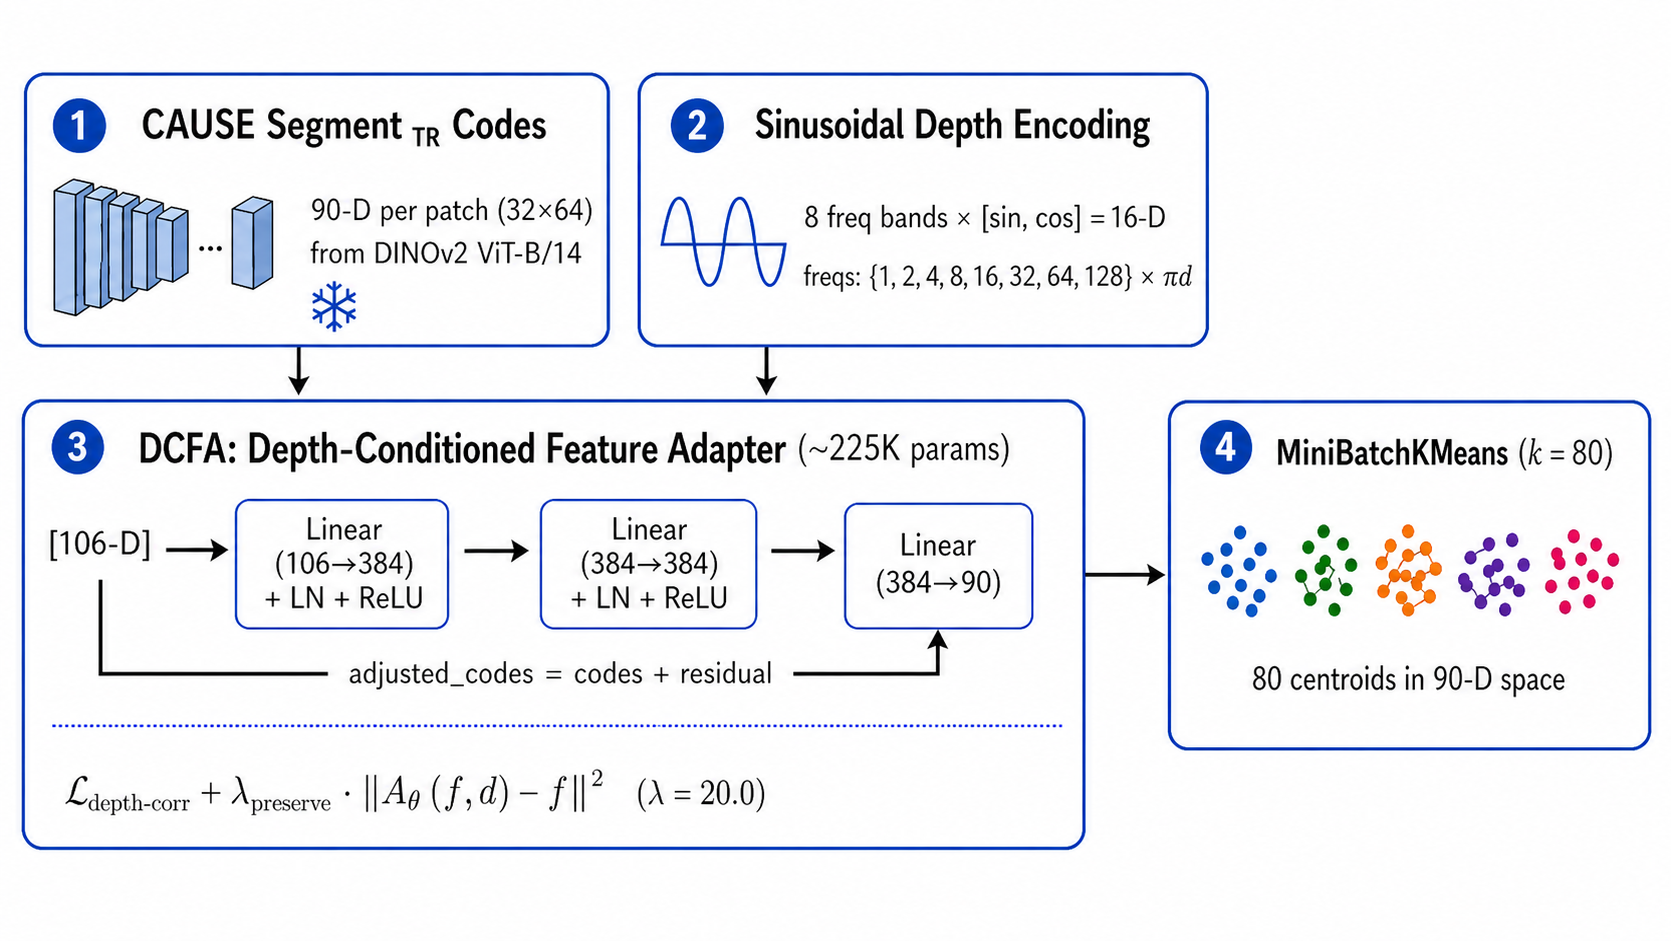
\includegraphics[width=\linewidth]{../figures/paper_ready/dcfa_adapter_training.png}
\caption{DCFA adapter training. A frozen CAUSE-TR~\cite{kim2024cause} code is adjusted by a depth-conditioned residual before $k$-means clustering, while a preservation term keeps the adapted code close to the original frozen semantic manifold.}
\label{fig:dcfa_adapter}
\end{figure}

The semantic regions inherited from the frozen CAUSE-TR~\cite{kim2024cause} code are appearance-driven, and the failure modes are: a single physical surface split across an illumination change, and two adjacent same-class objects merged into one region. Figure~\ref{fig:dcfa_adapter} summarizes the adapter path. We introduce a small residual adapter that consumes the depth value $d_u$ at pixel $u$ and adds a learned depth-driven shift to the frozen 90-dimensional code $z_u$, nudging cluster boundaries toward depth-consistent regions where appearance fails.

Conditioning on $d_u$ requires a representation rich enough for a small MLP to read both fine boundary differences and coarse depth ordering. Since $d_u \in [0, 1]$ is a scalar, we lift it through a 16-dimensional sinusoidal positional encoding with eight exponentially-spaced frequencies $\omega_k = 2^k \pi$ for $k = 0, \dots, 7$,
\begin{equation}
\begin{aligned}
e(d_u) = \big[ &\sin(\omega_0 d_u), \cos(\omega_0 d_u), \dots, \\
              &\sin(\omega_7 d_u), \cos(\omega_7 d_u) \big] \in \mathbb{R}^{16}.
\end{aligned}
\label{eq:sinusoid}
\end{equation}
The encoding $e(d_u)$ is concatenated with the frozen code $z_u$ into a 106-dimensional input, which a three-layer MLP $A: \mathbb{R}^{106} \to \mathbb{R}^{90}$ (two 384-wide hidden layers, each with layer normalization and ReLU, and a zero-initialized output projection) maps to a residual shift added to the frozen code,
\begin{equation}
\tilde z_u = z_u + A([z_u,\, e(d_u)]).
\label{eq:residual}
\end{equation}
The construction has approximately 225K (225,114) trainable parameters, small relative to the $\sim$86M parameters of the frozen ViT backbone. Two design choices keep the adapted code on the frozen CAUSE-TR~\cite{kim2024cause} manifold rather than re-learning a new representation: the output projection is zero-initialized, so that $\tilde z_u = z_u$ at the first optimizer step and any departure from the frozen code is acquired gradually through gradient descent; and the preservation term in Eq.~\ref{eq:dcfa_loss} with $\lambda_p = 20$ explicitly penalizes drift from $z_u$, so $\tilde z_u$ at convergence is a small, depth-conditioned perturbation of $z_u$ rather than an independently learned code.

Training the adapter calls for a self-supervised signal that pulls the adapted codes of pixels at similar depth toward each other while keeping them on the original CAUSE-TR~\cite{kim2024cause} manifold. DepthG~\cite{sick2024depthg} established that depth-feature correlation can guide unsupervised semantic learning when depth governs the loss; we apply the same loss to the adapted code rather than to the backbone weights. For each minibatch image, we sample 1024 pixels and 1024 pixel pairs, using the DepthG~\cite{sick2024depthg} depth-similarity kernel with bandwidth $\sigma_d = 0.5$. The adapter minimizes
\begin{equation}
\begin{aligned}
\mathcal{L}_\text{DCFA}
&= \mathcal{L}_\text{corr}(\tilde z, D)
 + \lambda_p \mathcal{L}_\text{preserve}(\tilde z, z), \\
\lambda_p &= 20 .
\end{aligned}
\label{eq:dcfa_loss}
\end{equation}
Let $\mathcal{U}$ denote the set of $|\mathcal{U}| = 1024$ pixels sampled per image and $\mathcal{P}$ the set of $|\mathcal{P}| = 1024$ pixel pairs sampled from $\mathcal{U}$. Then $\mathcal{L}_\text{corr} = \frac{1}{|\mathcal{P}|} \sum_{(i,j) \in \mathcal{P}} \mathcal{K}_{\sigma_d}(D_i, D_j)\,\big(1 - \cos(\tilde z_i, \tilde z_j)\big)$ is the DepthG~\cite{sick2024depthg} depth-similarity-weighted correlation loss with bandwidth $\sigma_d = 0.5$, and $\mathcal{L}_\text{preserve} = \frac{1}{|\mathcal{U}|} \sum_{u \in \mathcal{U}} \|\tilde z_u - z_u\|_2^2$ is the per-pixel mean squared distance between adapted and frozen codes over the same sampled set. Both losses average over the sampled set per image, then average over the minibatch.
\subsection{SIMCF: Semantic Instance Mutual Consistency Filtering}
\label{sec:method:simcf}

DCFA changes the feature space before clustering, but some errors remain after semantic and instance labels are formed. A depth fragment may cut through a single object, a proposal may contain pixels from multiple pseudo-classes, or a semantic assignment may sit at a depth far from the empirical range of its pseudo-class. SIMCF, short for Semantic Instance Mutual Consistency Filtering, is the final algorithm inside $G$: it takes the raw candidate pair $(S_x^0, I_x^0)$ and returns filtered pseudo-labels $(\hat S_x, \hat I_x)$ by enforcing consistency between semantic identity, instance geometry, feature similarity, and depth statistics.

Algorithm~\ref{alg:simcf} lists the procedure. The first check prevents mixed-class instance targets, the second repairs depth over-fragmentation using DINOv3 appearance similarity~\cite{simeoni2025dinov3}, and the third converts depth-implausible pixels into void labels rather than hard negatives. SIMCF is learning-free: it has no trainable parameters, and the four hyperparameters $\tau_\text{sim}$, $\eta$, $A_\text{min}$, and the 8-neighbour adjacency are fixed across all experiments and reported in Section~\ref{sec:exp:setup}. DCFA remains the only learned component inside the Stage-1 generator, and the filtered labels are passed directly to panoptic bootstrapping.

\begin{figure*}[t]
\centering
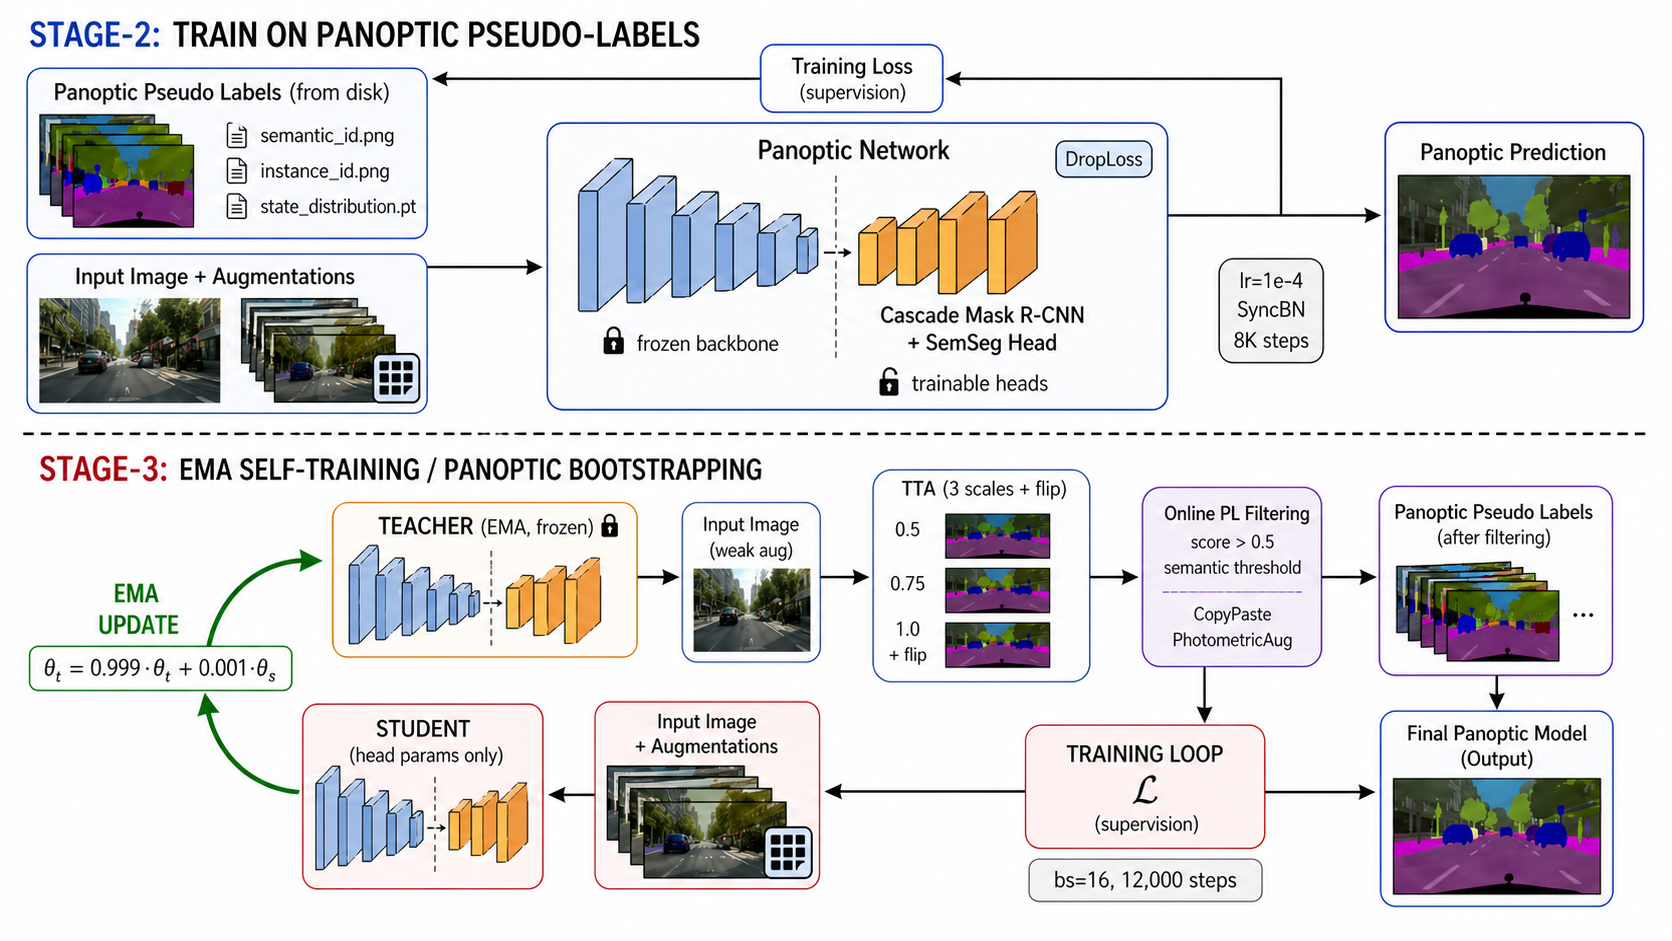
\includegraphics[width=0.90\textwidth]{../figures/paper_ready/panoptic_network_training.png}
\caption{Panoptic bootstrapping and panoptic network training. Filtered pseudo-labels supervise the initial panoptic network, and EMA self-training refines the labels and network across subsequent rounds, following the CUPS~\cite{hahn2025cups} training recipe.}
\label{fig:panoptic_training}
\end{figure*}

\subsection{Panoptic Bootstrapping and Panoptic Network Training}
\label{sec:method:detector}

Filtering completes the Stage-1 generator $G$. The resulting pseudo-labels $(\hat S_x, \hat I_x)$ provide the supervision for panoptic bootstrapping, while the RGB image $x$ remains the network input. Figure~\ref{fig:panoptic_training} shows the training path adopted from CUPS. We adopt the panoptic bootstrapping and panoptic network training procedures from CUPS~\cite{hahn2025cups}, including its loss, copy-paste augmentation, bootstrapping schedule, and EMA self-training. Keeping these procedures fixed across configurations lets the experiments isolate the effect of the pseudo-label source.

The panoptic network takes $x$ as input and is trained on $(\hat S_x, \hat I_x)$. Its cascade, proposal, and panoptic heads use the CUPS-style~\cite{hahn2025cups} losses; Section~\ref{sec:exp:setup} specifies the architecture.

\begin{cvpralgorithm}
\algorithmcaption{SIMCF$(S_x^0,I_x^0,D,\phi,v;\tau_\text{sim},\eta)$.}
\label{alg:simcf}
\begin{enumerate}
\setlength{\itemsep}{0pt}
\setlength{\topsep}{2pt}
\item $(\hat S_x,\hat I_x) \gets (S_x^0,I_x^0)$
\item \algkw{for each} instance region $R_k=\{p:\hat I_x(p)=k\}$ \algkw{do}
\item \algindent $c_k \gets \arg\max_c |\{p\in R_k:\phi(\hat S_x(p))=c\}|$
\item \algindent $s_k \gets \arg\max_s |\{p\in R_k:\hat S_x(p)=s,\ \phi(s)=c_k\}|$
\item \algindent \algkw{for each} $p\in R_k$ with $\phi(\hat S_x(p))\ne c_k$ \algkw{do}
\item \algindenttwo $\hat S_x(p)\gets s_k$
\item \algkw{for each} adjacent proposal pair $(a,b)$ in $\hat I_x$ \algkw{do}
\item \algindent compute mean features $\bar v_a,\bar v_b$ over $R_a,R_b$
\item \algindent \algkw{if} $c_a=c_b$ and $\cos(\bar v_a,\bar v_b)>\tau_\text{sim}$ \algkw{then}
\item \algindenttwo merge $R_a$ and $R_b$ in $\hat I_x$
\item \algkw{for each} pseudo-class $c$ \algkw{do}
\item \algindent $P_c\gets\{p:\phi(\hat S_x(p))=c\}$
\item \algindent $(\mu_c,\sigma_c)\gets(\operatorname{mean}D(P_c),\operatorname{std}D(P_c))$
\item \algkw{for each} pixel $p$ \algkw{do}
\item \algindent $c\gets\phi(\hat S_x(p))$
\item \algindent \algkw{if} $|D(p)-\mu_c|>\eta\sigma_c$ \algkw{then}
\item \algindenttwo $\hat S_x(p)\gets\mathrm{void}$; \quad $\hat I_x(p)\gets0$
\item \algkw{return} $(\hat S_x,\hat I_x)$
\end{enumerate}
\end{cvpralgorithm}

Two ingredients of the inherited recipe interact directly with the void labels produced by SIMCF. Following CUPS~\cite{hahn2025cups}, DropLoss~\cite{wang2023cutler} masks losses on void or unreliable regions so that rejected pseudo-labels are not treated as hard negatives, making void a soft abstention rather than a class signal. Self-enhanced copy-paste augmentation operates at the input level: at each training iteration, instances from the pseudo-labels of one image are pasted into another image at random positions. This augmentation increases exposure to thing-class instances.

Once the cascade trainer reaches its bootstrapped checkpoint, three rounds of EMA self-training continue from it. In each round, an exponential-moving-average teacher is maintained over the student weights and used to relabel the unlabeled training set; the student is re-trained on the resulting refined pseudo-labels. The teacher provides a smoother, lower-variance label distribution than $G$ alone supplies, in particular for thing-class boundaries where Stage-1 labels are limited by monocular depth discontinuities. We use the final-round student checkpoint as the network $F$ in Eq.~\ref{eq:pipeline}.

At test time, $F$ produces a panoptic prediction $(S_x, I_x)$ via the standard panoptic merge of~\cite{kirillov2019panoptic} applied to its dense semantic output and cascade instance proposals. Two design choices are non-obvious. First, $F$ predicts directly into the pseudo-class vocabulary on which it was trained, not into the 27-class Cityscapes taxonomy: the Hungarian mapping from pseudo-classes to benchmark classes is computed only at evaluation time and is the only ground-truth-derived component anywhere in the pipeline; neither $G$ nor $F$ ever consults benchmark labels during training. Second, the thing/stuff partition that drives the merge is inherited from the frozen CAUSE-TR~\cite{kim2024cause} taxonomy (§\ref{sec:method:baseline}), not from the evaluation taxonomy, so the same partition supervises Stage-1 instance extraction and Stage-3 panoptic merging without taxonomy drift across stages.

Figure~\ref{fig:real_data_flow} traces the same data flow on real Cityscapes images, showing Stage-1 intermediate outputs together with the paired RGB/label transformations used by panoptic bootstrapping and panoptic network training.

\begin{figure*}[!t]
\centering
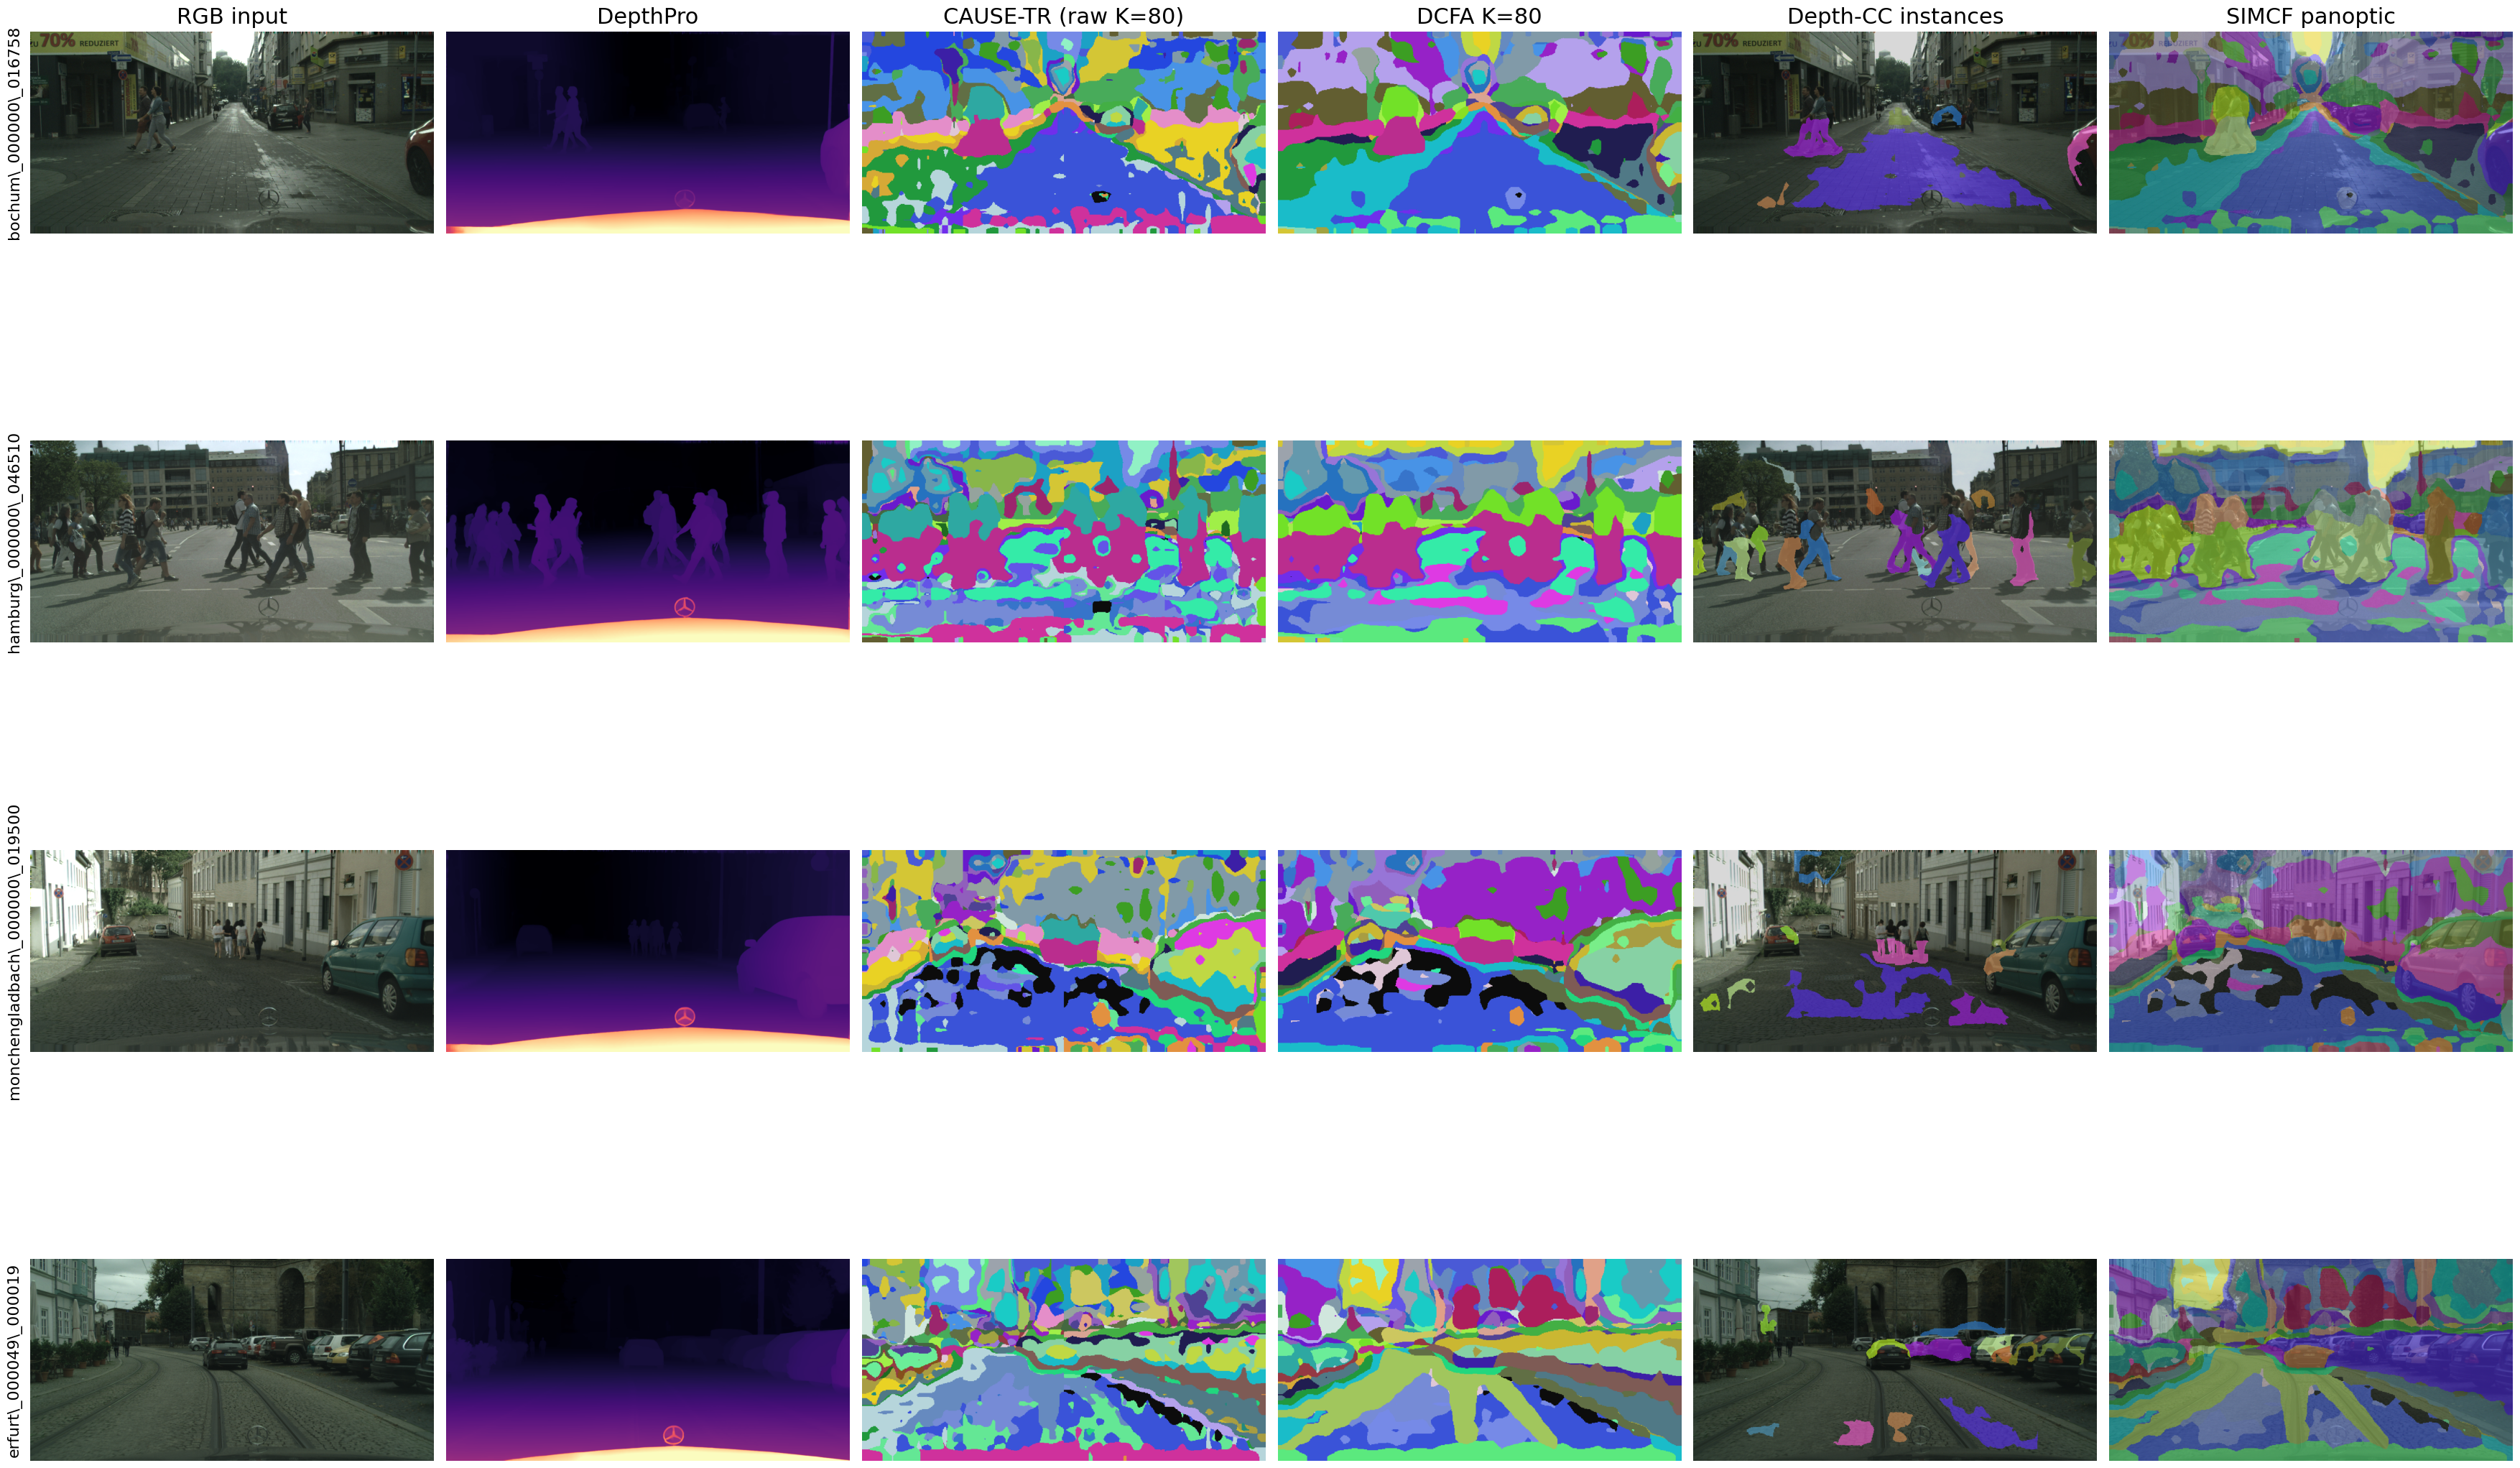
\includegraphics[width=\textwidth]{../figures/paper_ready/fig5_stage1_trace_composite.png}
\caption{Stage-1 pseudo-label trace on four Cityscapes train frames. Columns: RGB; DepthPro depth; CAUSE-TR~\cite{kim2024cause} raw $K{=}80$ clusters; DCFA-adjusted $K{=}80$; depth-CC instances on RGB; final SIMCF-filtered panoptic pseudo-labels on RGB. Row 2 (hamburg) is the canonical co-planar pedestrian failure case (Section~\ref{sec:discussion}, Section~\ref{sec:limitations}).}
\label{fig:real_data_flow}
\end{figure*}

%=========================================================================
\section{Experiments}
\label{sec:experiments}
%=========================================================================

We report experiments on Cityscapes and zero-shot transfer datasets, separating pseudo-label quality from trained-network performance. The evaluation asks whether monocular pseudo-labels can seed the adopted CUPS~\cite{hahn2025cups} training procedure, how much DCFA and SIMCF contribute, and where the fixed Cityscapes-derived pseudo-class vocabulary fails.

\subsection{Experimental Setup}
\label{sec:exp:setup}

Pseudo-label generation and panoptic network training use only Cityscapes train~\cite{cordts2016cityscapes} (2,975 images, no annotations); evaluation reports Cityscapes val (500 images) under the 27-class CAUSE~\cite{kim2024cause} pseudo-vocabulary with a Hungarian map to the 27-class Cityscapes label space (\texttt{NUM\_CLASSES=27} in the official CUPS protocol~\cite{hahn2025cups}; this is the full Cityscapes label space, including parking, rail track, guard rail, bridge, tunnel, polegroup, caravan, and trailer in addition to the 19 standard semantic-segmentation classes). The Stage-1 generator $G$ uses a frozen DINOv2 ViT-B/14 backbone~\cite{oquab2024dinov2}, the frozen CAUSE-TR head~\cite{kim2024cause}, DCFA ($h = 384$, 16-D sinusoidal depth embedding, $\lambda_\text{preserve} = 20$, $\sim$225K trainable parameters trained for 10K optimizer iterations with AdamW at learning rate $10^{-3}$, batch size 32 images, sampling 1024 pixels and 1024 pixel pairs per image), $k$-means over-clustering at $k = 80$, the Section~\ref{sec:method:baseline} monocular instance branch with $\tau_d = 0.20$, $A_\text{min} = 1000$, and three iterations of dilation, and SIMCF ($\tau_\text{sim} = 0.85$, $\eta = 2.5$). DepthPro~\cite{bochkovskii2024depthpro} supplies the monocular depth map.

The operating hyperparameters ($k=80$, $A_\text{min}=1000$, $\tau_d=0.20$, $\tau_\text{sim}=0.85$, $\eta=2.5$, and $\lambda_p=20$) were fixed before consulting Cityscapes annotations. The SIMCF sweep in Table~\ref{tab:simcf_sensitivity} is a retrospective sensitivity analysis, not a model-selection procedure.

We follow CUPS~\cite{hahn2025cups} for the training side. Panoptic bootstrapping denotes the initial training of a panoptic network on Stage-1 pseudo-labels with DropLoss~\cite{wang2023cutler} and self-enhanced copy-paste augmentation. Panoptic network training denotes the subsequent EMA self-training rounds, where teacher predictions relabel the training set and the student continues training on the refined labels. In both stages, the panoptic network is a Cascade Mask R-CNN~\cite{cai2018cascade} with three cascade stages on a frozen DINOv3 ViT-B/16 backbone~\cite{simeoni2025dinov3}; we use 8K bootstrapping steps followed by three 5K-step EMA rounds with EMA coefficient 0.999 and a three-scale teacher. All training is performed on $2 \times$ NVIDIA GTX 1080 Ti GPUs with PyTorch DistributedDataParallel: Stage-2 panoptic bootstrapping completes in $\approx 12$ hours and the three Stage-3 EMA rounds complete in $\approx 16$ hours, for a total of $\approx 28$ GPU-hours per machine ($\approx 56$ GPU-hours aggregate). Stage-1 pseudo-label generation, including DCFA training (10K iterations, $\sim$1 hour) and SIMCF filtering, runs once per dataset and adds $\approx 2$ further GPU-hours. The whole pipeline is therefore feasible on consumer-grade hardware that lacks the calibrated stereo rigs and synchronized video required by CUPS~\cite{hahn2025cups} at pseudo-label time.


\subsection{Main Cityscapes Results}
\label{sec:exp:main}

Table~\ref{tab:main} records two comparisons on Cityscapes val: published external references, including CUPS~\cite{hahn2025cups}, and an in-paper controlled comparison that holds the Stage-2/3 trainer fixed. Our method reaches 35.83 PQ, a $+$3.07 PQ gain over the matched monocular baseline and a $+$8.03 PQ gain over the published stereo+flow CUPS reference~\cite{hahn2025cups} under the reported CUPS evaluation protocol~\cite{hahn2025cups} ($+$5.39 SQ, $+$8.58 RQ, $+$18.56 PQ$^\text{Th}$, $+$0.46 PQ$^\text{St}$). The supervised row (62.3 PQ) is an oracle upper bound.

The two ``ours'' rows isolate the contribution of DCFA$+$SIMCF: both share the same Stage-2/3 recipe, identical panoptic bootstrapping and EMA self-training, and identical Cascade Mask R-CNN backbone; only the Stage-1 pseudo-label source differs. The monocular baseline is trained on raw $K$=80 pseudo-labels (24.54 pseudo-PQ), without DCFA or SIMCF, with Stage-1 inputs differing only in (a) raw 90-D CAUSE-TR~\cite{kim2024cause} semantic code (no DCFA residual), and (b) DepthPro connected components at $\tau_d = 0.20$ with no SIMCF filtering. DCFA$+$SIMCF add $+$3.07 PQ to the trained-network result in this controlled comparison.

\begin{table*}[t]
\centering
\small
\setlength{\tabcolsep}{3pt}
\begin{tabular}{l l l c c c c c c}
\toprule
Method & Training data & PL inputs & Eval cls. & PQ & SQ & RQ & PQ$^\text{Th}$ & PQ$^\text{St}$ \\
\midrule
\rowcolor{black!5} Supervised~\cite{kirillov2019panoptic} & CS & dense labels & -- & 62.3 & 81.8 & 75.1 & 62.4 & 62.1 \\
\midrule
DepthG~\cite{sick2024depthg}$+$CutLER~\cite{wang2023cutler} & CS \& ImageNet & RGB mono. & 27 & 16.1 & 45.4 & 21.1 & \phantom{0}3.0 & 25.7 \\
U2Seg~\cite{niu2024u2seg} & COCO \& ImageNet & RGB mono. & 800$+$27 & 18.4 & 55.8 & 22.7 & 10.2 & 24.3 \\
S2-UniSeg~\cite{xu2025s2uniseg} & SA-1B \& CS & RGB mono. & -- & 25.4 & 66.7 & 35.0 & -- & -- \\
CUPS~\cite{hahn2025cups} & CS & RGB$+$stereo$+$flow & 27 & 27.80 & 57.4 & 35.2 & 17.7 & 35.1 \\
\midrule
Monocular baseline (no DCFA/SIMCF) & CS & RGB mono. & 27 & 32.76 & 62.57 & 40.75 & -- & -- \\
\textbf{Ours (DCFA$+$SIMCF)} & CS & RGB mono. & 27 & \textbf{35.83} & \textbf{62.79} & \textbf{43.78} & \textbf{36.26} & \textbf{35.56} \\
\midrule
\textit{vs.\ CUPS~\cite{hahn2025cups}} (prev.\ scene-centric SOTA) & & & & \textcolor{green!50!black}{$+$8.03} & \textcolor{green!50!black}{$+$5.39} & \textcolor{green!50!black}{$+$8.58} & \textcolor{green!50!black}{$+$18.56} & \textcolor{green!50!black}{$+$0.46} \\
\bottomrule
\end{tabular}
\caption{Unsupervised panoptic segmentation on Cityscapes val (all in \%, $\uparrow$). ``PL inputs'' are the inputs available at pseudo-label time. ``Eval cls.'' is the number of benchmark classes used by the CUPS~\cite{hahn2025cups} evaluation protocol; our network predicts $K{=}80$ pseudo-classes and is aligned to the 27-class taxonomy only at metric time (Section~\ref{sec:exp:setup}).}
\label{tab:main}
\end{table*}

The final model after Stage-2 panoptic bootstrapping and three rounds of Stage-3 EMA self-training reaches 35.83 PQ, 62.79 SQ, and 43.78 RQ on Cityscapes val. The improvement over the pseudo-label generator is concentrated in recognition rather than mask quality, indicating that the panoptic bootstrapping and EMA self-training stages principally amplify class recall while preserving the mask geometry already produced by the Stage-1 generator. The trained-model mIoU of 44.56\% is reported under the 19-class semantic-segmentation evaluation taxonomy used historically for unsupervised mIoU comparison.

The aggregate gain is not uniform: large stuff regions and large vehicles combine high SQ with high RQ, while thin structures and rare classes are recognition-limited. The full per-class breakdown is deferred to Table~\ref{tab:perclass} in Section~\ref{sec:exp:generalization}, where it is interpreted alongside the failure analysis.

Figure~\ref{fig:qualitative_stage3} shows representative panoptic predictions from the trained Stage-3 network on nine Cityscapes val images, none of which were used for training. Each row presents the input RGB, the panoptic prediction colorized in the $K=80$ pseudo-class space, and the prediction overlaid on the input.

\begin{figure*}[t]
\centering
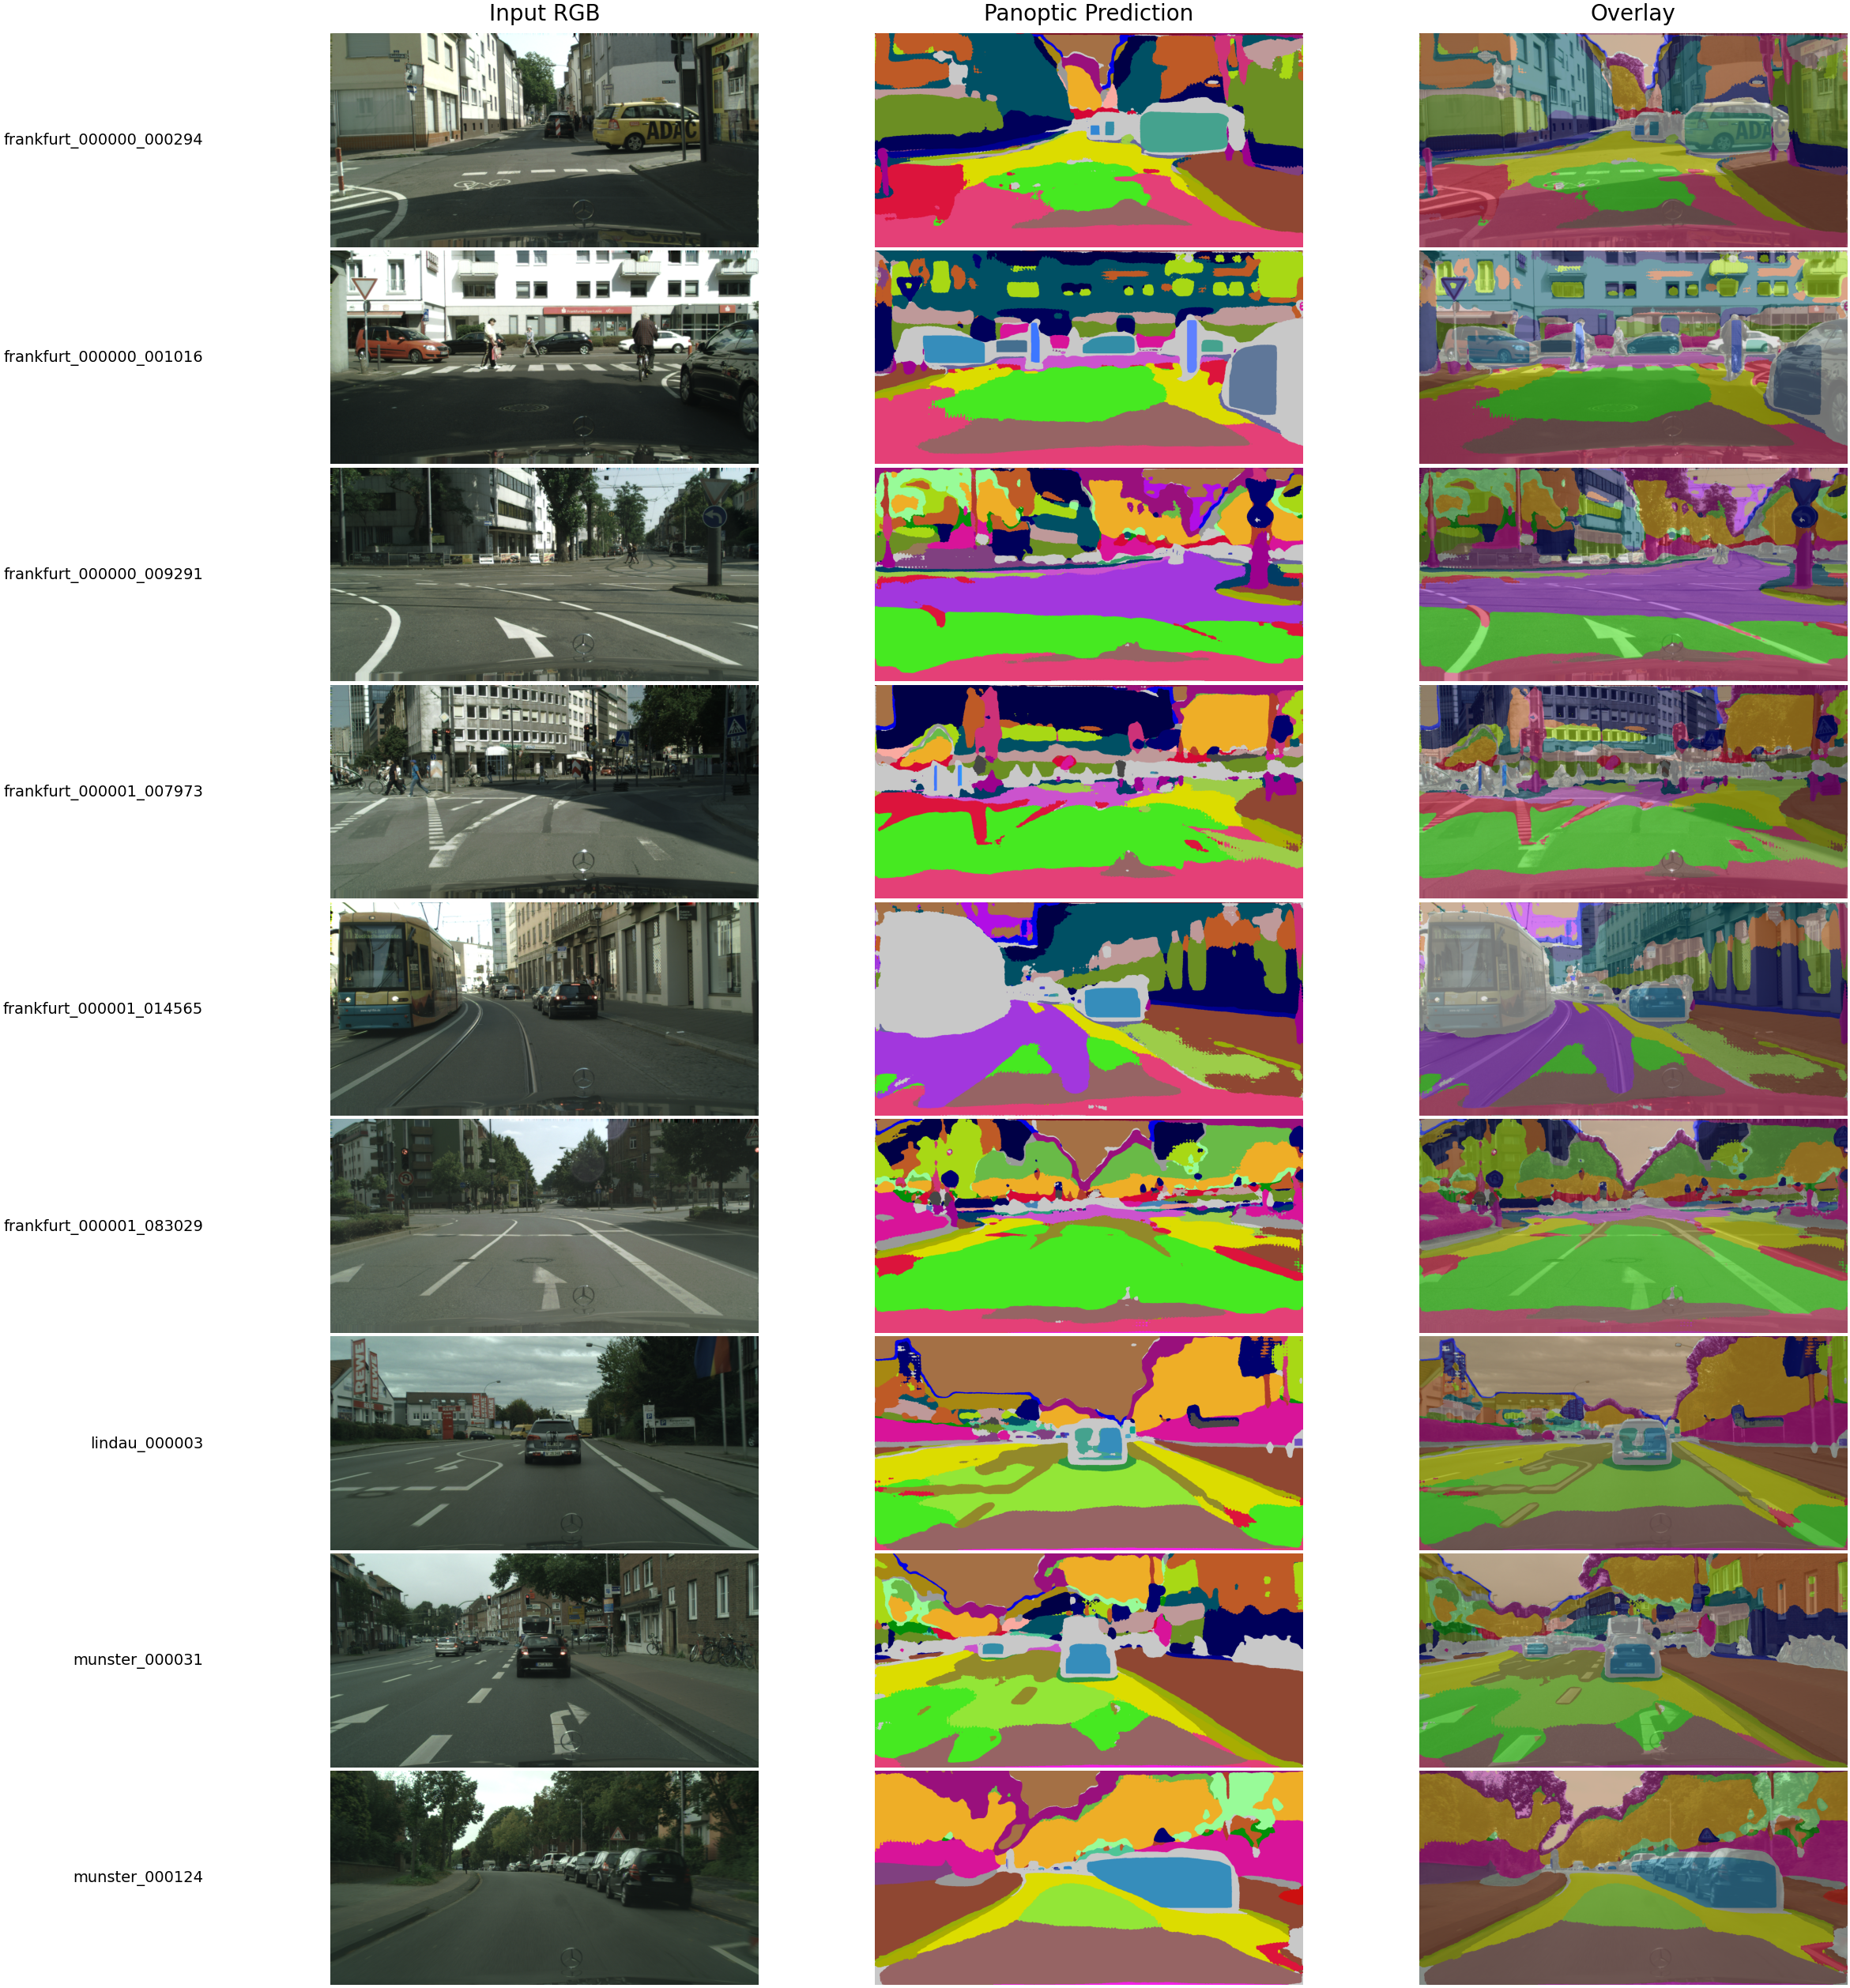
\includegraphics[width=0.96\linewidth]{../figures/paper_ready/qualitative_stage3.png}
\caption{Stage-3 panoptic predictions on Cityscapes val (9 held-out images). Columns: RGB input, panoptic prediction in the $K=80$ pseudo-class space, RGB overlay ($\alpha{=}0.55$). Hungarian alignment to the 27-class Cityscapes evaluation taxonomy is computed only at metric time and is not applied here, so colors track pseudo-class IDs rather than benchmark classes. Light grey marks pixels that the network rejects below its semantic confidence threshold (void).}
\label{fig:qualitative_stage3}
\end{figure*}


\subsection{Ablations}
\label{sec:exp:ablations}

\paragraph{Pipeline progression.}
Table~\ref{tab:progression} traces how PQ accumulates across the four pipeline stages. Stage-1 raw pseudo-labels reach 24.54 PQ; adding our two Stage-1 contributions (DCFA + SIMCF) lifts pseudo-label PQ to 25.85 ($+1.31$). Stage-2 panoptic bootstrapping then trains a Cascade Mask R-CNN on these pseudo-labels and reaches 28.40 PQ, and Stage-3 EMA self-training carries the network to its final \textbf{35.83 PQ} on Cityscapes val. Two observations follow. First, every stage of the pipeline contributes a meaningful uplift; the largest single jump is the trained-network step, which converts pseudo-label structure into recognition recall. Second, the contribution of DCFA+SIMCF compounds through training: the $+1.31$ PQ Stage-1 advantage grows to $+3.07$ PQ at the trained-network level, indicating that better pseudo-labels are not only better at pseudo-label time but also amplify under the Stage-2/3 procedure.

\begin{table}[t]
\centering
\small
\setlength{\tabcolsep}{3pt}
\begin{tabular}{l l c}
\toprule
\# & Pipeline stage & PQ \\
\midrule
1 & Stage-1 pseudo-labels (raw, no DCFA, no SIMCF) & 24.54 \\
2 & \quad $+$ DCFA $+$ SIMCF (our Stage-1 contributions) & 25.85 \\
3 & \quad $+$ Stage-2 panoptic bootstrapping & 28.40 \\
4 & \quad $+$ Stage-3 EMA self-training (final) & \textbf{35.83} \\
\bottomrule
\end{tabular}
\caption{Pipeline progression on Cityscapes val. Each row adds one component to the row above.}
\label{tab:progression}
\end{table}

\paragraph{Component contribution.}
Table~\ref{tab:components} reports DCFA $\times$ SIMCF at the fixed training-data instance configuration ($\tau_d = 0.20$). All four cells share the same depth instances; only the pre-clustering adapter and the post-instance filter are toggled. The load-bearing observation is the +1.31 PQ jump from Raw $K$=80 (24.54) to Both (25.85), and the +0.58/+0.63 PQ separation between Both and either single component, which is consistent with the two corrections targeting different failure modes (DCFA reshapes the feature space, SIMCF filters the resulting labels) and combining super-additively. The single-component rows DCFA-only (25.22) and SIMCF-only (25.27) are within 0.05 PQ of each other and should not be read as a strict ordering between the two mechanisms; the relevant claim is complementarity, evidenced by the move from either single component to Both.

\begin{table}[t]
\centering
\small
\setlength{\tabcolsep}{3pt}
\begin{tabular}{l c c c c c c}
\toprule
Variant & DCFA & SIMCF & PQ & SQ & RQ & mIoU \\
\midrule
Raw $K$=80 & -- & -- & 24.54 & 60.0 & 33.6 & 52.69 \\
DCFA only & \checkmark & -- & 25.22 & 61.0 & 34.0 & 55.29 \\
SIMCF only & -- & \checkmark & 25.27 & 57.5 & 34.4 & 52.69 \\
Both & \checkmark & \checkmark & 25.85 & 58.3 & 34.9 & 55.29 \\
\bottomrule
\end{tabular}
\caption{Pseudo-label component complementarity at fixed $\tau_d = 0.20$ DepthPro instances. ``Raw $K$=80'' is the no-DCFA, no-SIMCF baseline. mIoU is the Cityscapes val 19-class semantic-segmentation mIoU; SIMCF filters instance proposals and does not modify the semantic prediction, so the SIMCF-only and DCFA$+$SIMCF rows inherit the mIoU of the underlying semantic code.}
\label{tab:components}
\end{table}

\paragraph{SIMCF threshold sensitivity.}
SIMCF exposes two thresholds: $\tau_\text{sim}$ for adjacent-proposal feature merging (Step B) and $\eta$ for depth-implausibility void rejection (Step C). To verify that SIMCF's contribution is not the product of threshold tuning, we sweep both $\pm$$\sim$$12\%$ around the paper setting and re-evaluate pseudo-label quality on the full Cityscapes train set ($N=2975$). Table~\ref{tab:simcf_sensitivity} reports the result. Pseudo-label PQ varies within a 0.71-point band (25.27--25.98) across the sweep, smaller than the +1.31 PQ super-additive gap from either single component to Both reported in Table~\ref{tab:components}. Tighter thresholds slightly improve PQ (more aggressive merging recovers more depth over-fragmentations); looser thresholds degrade modestly. The mechanism is therefore robust to moderate threshold perturbation rather than tuned-on-test.

\begin{table}[t]
\centering
\small
\setlength{\tabcolsep}{3pt}
\begin{tabular}{l c c c c c c}
\toprule
Setting & $\tau_\text{sim}$ & $\eta$ & PQ & SQ & RQ & mIoU \\
\midrule
tighter         & 0.75 & 2.0 & 25.98 & 58.79 & 34.55 & 56.08 \\
baseline (paper) & 0.85 & 2.5 & 25.87 & 58.38 & 34.83 & 56.17 \\
looser          & 0.95 & 3.0 & 25.27 & 57.63 & 34.10 & 56.22 \\
\bottomrule
\end{tabular}
\caption{SIMCF threshold sensitivity at fixed depth instances ($\tau_d=0.20$, DepthPro). Pseudo-label PQ is computed on the full Cityscapes train set under the CUPS~\cite{hahn2025cups} 27-class protocol; discussed in Section~\ref{sec:exp:ablations}.}
\label{tab:simcf_sensitivity}
\end{table}

\paragraph{DCFA conditioning mechanism.}
The novelty claim in Section~\ref{sec:related} contrasts DCFA's architectural depth conditioning with DepthG-style~\cite{sick2024depthg} loss-side conditioning. We separate the contribution of the two axes empirically (Table~\ref{tab:conditioning}). \emph{DepthG~\cite{sick2024depthg} (drop-in)} loads the official DepthG checkpoint~\cite{sick2024depthg} (DINO ViT-B/8 + STEGO-style cluster head trained with depth-correlation loss on Cityscapes train, $\dim{=}100$, ZoeDepth) and uses it as a Stage-1 generator under our identical downstream pipeline (k-means $k$=80, DepthPro depth-CC instances, eval). \emph{Loss-side $P(z)$} replaces DCFA's depth-conditioned residual with a learnable projection $P : \mathbb{R}^{90} \to \mathbb{R}^{90}$ ($P(z) = z + \text{MLP}(z)$, 70K parameters, no depth as architectural input) trained on cached CAUSE~\cite{kim2024cause} codes with only the depth-correlation loss $\mathcal{L}_\text{corr}(P(z), D)$. We further isolate the preservation axis with \emph{Loss-side $P(z)$ + preserve}, which adds $\lambda_p \mathcal{L}_\text{preserve}$ ($\lambda_p=20$) to the loss-side objective.

The decomposition reads as follows. Without preservation, both loss-side methods collapse far below the raw baseline (DepthG~\cite{sick2024depthg} drop-in $-11.21$ PQ; loss-side without preserve $-11.92$ PQ), confirming that any unconstrained re-shaping of a frozen unsupervised concept-clusterbook code degrades the embedding structure that downstream $k$-means relies on. Adding preservation rescues most of the structure (loss-side with preserve reaches 23.83 PQ), but is still $-0.71$ PQ below the raw baseline and $-1.39$ PQ below DCFA. The remaining $+1.39$ PQ gap between loss-side+preserve and DCFA, at matched parameter budget and matched preservation strength, is the empirical contribution of \emph{architectural} depth conditioning -- depth as an input to the conditioning network, not just to the loss. The two axes -- architectural input and explicit manifold preservation -- are both required for the $+0.68$ PQ over raw, and neither is a strict substitute for the other.

\begin{table}[t]
\centering
\scriptsize
\setlength{\tabcolsep}{3pt}
\begin{tabular}{@{}l l c c c c@{}}
\toprule
Method & Conditioning & PQ & SQ & RQ & mIoU \\
\midrule
Raw $K$=80 (paper substrate)        & none                  & 24.54 & 60.00 & 33.60 & 52.69 \\
DepthG~\cite{sick2024depthg} (official, ViT-B/8)          & loss, end-to-end      & 13.33 & 33.39 & 18.56 & -- \\
Loss-side $P(z)$ on CAUSE~\cite{kim2024cause}           & loss, no preserve     & 12.62 & 55.35 & 18.95 & -- \\
Loss-side $P(z)$ + preserve         & loss $+$ preserve     & 23.83 & 56.54 & 32.76 & -- \\
DCFA (ours)                         & residual $+$ preserve & \textbf{25.22} & \textbf{61.00} & \textbf{34.00} & \textbf{55.29} \\
\bottomrule
\end{tabular}
\caption{Conditioning-mechanism decomposition at the Stage-1 pseudo-label level (Section~\ref{sec:exp:ablations}). All rows share the same downstream pipeline; only how depth enters the model varies.}
\label{tab:conditioning}
\end{table}

\paragraph{Depth model.}
Table~\ref{tab:depth} reports representative depth-source and threshold runs for which the evaluations provide aggregate SQ and RQ. The rows are not used as a single leaderboard because some runs use the raw $K$=80 semantic map and others use the DCFA semantic map; they are used to separate mask quality from recognition quality while choosing the training-data configuration.

\begin{table}[t]
\centering
\small
\setlength{\tabcolsep}{3pt}
\begin{tabular}{l l c c c c}
\toprule
Depth & Sem. & $\tau$ & PQ & SQ & RQ \\
\midrule
SPIdepth & raw $K$=80 & 0.20 & 26.74 & 71.88 & 31.41 \\
DA v3~\cite{lin2025da3} & raw $K$=80 & 0.03 & 27.37 & 73.44 & 35.66 \\
DA v3~\cite{lin2025da3} & DCFA & 0.20 & 26.44 & 61.37 & 35.83 \\
DepthPro~\cite{bochkovskii2024depthpro} & DCFA & 0.01 & 27.81 & 63.07 & 37.40 \\
DepthPro~\cite{bochkovskii2024depthpro} & DCFA & 0.20 & 26.13 & 60.63 & 35.80 \\
\bottomrule
\end{tabular}
\caption{Depth and threshold diagnostics with aggregate SQ/RQ.}
\label{tab:depth}
\end{table}

The table shows why PQ alone is not a sufficient diagnostic for the depth branch. The sharper $\tau = 0.01$ DepthPro setting has stronger standalone PQ/SQ/RQ, but it produces a fragmented training set with roughly 57 instances per image and more than half below 1000 pixels. The $\tau = 0.20$ setting has lower standalone PQ but produces larger training targets, roughly 22 instances per image, which is the configuration used for panoptic bootstrapping. DA v3 at the same training-data threshold reaches a similar RQ, indicating that the choice is governed by the training signal produced by the depth branch rather than by the stuff/thing aggregate split.


\subsection{Generalization and Failure Analysis}
\label{sec:exp:generalization}

\begin{table*}[t]
\centering
\footnotesize
\setlength{\tabcolsep}{4pt}
\begin{tabular}{l c c c c c c c c c}
\toprule
\multirow{2}{*}{Method} & \multicolumn{3}{c}{KITTI~\cite{geiger2012kitti}} & \multicolumn{3}{c}{Waymo V2~\cite{sun2020waymo}$^{\P}$} & \multicolumn{3}{c}{Mapillary v2$^{\dagger}$} \\
\cmidrule(lr){2-4} \cmidrule(lr){5-7} \cmidrule(lr){8-10}
& PQ & SQ & RQ & PQ & SQ & RQ & PQ & SQ & RQ \\
\midrule
\rowcolor{black!5} Supervised~\cite{kirillov2019panoptic} & 31.9 & 71.7 & 40.4 & 31.5 & 70.1 & 40.9 & -- & -- & -- \\
\midrule
DepthG~\cite{sick2024depthg}$+$CutLER~\cite{wang2023cutler} & 11.0 & 34.5 & 13.8 & 13.4 & 37.3 & 17.0 & -- & -- & -- \\
U2Seg~\cite{niu2024u2seg} & 20.6 & 52.9 & 25.2 & 19.8 & 50.8 & 23.4 & -- & -- & -- \\
CUPS~\cite{hahn2025cups} & 25.5 & 58.1 & 32.5 & 26.4 & 60.3 & 33.0 & -- & -- & -- \\
\midrule
\textbf{Ours (DCFA$+$SIMCF), 19-class}$^{\S}$ & \textbf{34.85} & \textbf{62.43} & \textbf{42.91} & \textbf{43.51} & \textbf{76.82} & \textbf{50.54} & \textbf{39.19} & \textbf{74.59} & \textbf{47.74} \\
\textbf{Ours (DCFA$+$SIMCF), 27-class}$^{\S}$ & \textbf{34.85} & \textbf{62.43} & \textbf{42.91} & -- & -- & -- & \textbf{27.79} & \textbf{59.64} & \textbf{35.43} \\
\midrule
\textit{vs.\ CUPS~\cite{hahn2025cups}} & \textcolor{green!50!black}{$+$9.4} & \textcolor{green!50!black}{$+$4.3} & \textcolor{green!50!black}{$+$10.4} & \textcolor{green!50!black}{$+$17.1} & \textcolor{green!50!black}{$+$16.5} & \textcolor{green!50!black}{$+$17.5} & -- & -- & -- \\
\bottomrule
\end{tabular}
\caption{Cross-dataset generalization on driving-scene benchmarks (PQ/SQ/RQ in \%, $\uparrow$). Published baselines from~\cite{hahn2025cups}~Tab.~2. ``--'' marks datasets a baseline does not report. $^{\S}$KITTI 19-class and 27-class are identical (KITTI GT only contains the 19 standard classes); $^{\P}$Waymo via CUPS~\cite{hahn2025cups} Waymo loader; $^{\dagger}$Mapillary via paper-defined remap. Protocol details and OOD sanity (Table~\ref{tab:cocooo}) discussed in Section~\ref{sec:exp:generalization}.}
\label{tab:transfer}
\end{table*}

\begin{table}[t]
\centering
\footnotesize
\setlength{\tabcolsep}{3pt}
\begin{tabular}{l c c c c}
\toprule
Dataset (OOD) & \# img & PQ & SQ & RQ \\
\midrule
MOTS~\cite{voigtlaender2019mots} thing-only & 2{,}862 & 61.10 & 88.71 & 65.80 \\
\quad CUPS~\cite{hahn2025cups} ref. & --- & 86.4 & 86.4 & 76.9 \\
COCO-Stuff-27~\cite{caesar2018coco} vocab.\ mismatch & 1{,}000 & \phantom{0}7.83 & 38.55 & 10.06 \\
\bottomrule
\end{tabular}
\caption{Out-of-distribution sanity checks on a thing-only label space (MOTS) and a vocabulary-mismatched object-centric dataset (COCO-Stuff-27). Discussed in Section~\ref{sec:exp:generalization}.}
\label{tab:cocooo}
\end{table}

Our trained network transfers across the driving class space without retraining. KITTI reaches 34.85 PQ, surpassing CUPS~\cite{hahn2025cups} by $+$9.35 PQ; Waymo V2 reaches 43.51 PQ, surpassing CUPS~\cite{hahn2025cups} by $+$17.11 PQ; Mapillary v2 reaches 39.19 PQ. We report each dataset under the 19-class CUPS cross-dataset protocol~\cite{hahn2025cups} used by CUPS for KITTI, and report KITTI and Mapillary again under the 27-class CUPS in-domain protocol~\cite{hahn2025cups} for paper-internal consistency (Table~\ref{tab:transfer}). KITTI's panoptic ground truth contains only the 19 standard Cityscapes classes, so 19-class and 27-class evaluations yield identical numbers (34.85 PQ in either taxonomy). Mapillary contains ground truth for all eight Cityscapes-27 extras and is genuinely protocol-sensitive: 27-class PQ is 27.79 because eight low-coverage extras (parking, rail track, guard rail, bridge, tunnel, polegroup, caravan, trailer; 4.42\% of GT pixels combined) enter the average rather than mapping to void. Waymo V2 is evaluated through the CUPS Waymo pathway~\cite{hahn2025cups}, which maps raw Waymo panoptic labels to Cityscapes-19 over the 16 supported classes. Out-of-distribution sanity checks (MOTS thing-only and COCO-Stuff-27 vocabulary-mismatch) are reported in Table~\ref{tab:cocooo}; COCO-Stuff-27 (7.83 PQ) is dominated by categories absent from a Cityscapes-derived pseudo-label space and indicates the vocabulary boundary of in-domain training rather than a transfer failure of the architecture.

\paragraph{Per-class failure analysis.}
\begin{table*}[t]
\centering
\small
\setlength{\tabcolsep}{6pt}
\begin{tabular}{l c c c l c c c l c c c}
\toprule
Class & PQ & SQ & RQ & Class & PQ & SQ & RQ & Class & PQ & SQ & RQ \\
\midrule
road & 93.0 & 95.0 & 97.9 & tunnel & 0.0 & 0.0 & 0.0 & rider & 22.9 & 62.6 & 36.6 \\
sidewalk & 62.4 & 78.5 & 79.5 & pole & 2.0 & 72.3 & 2.8 & car & 70.7 & 88.7 & 79.7 \\
parking & 0.0 & 0.0 & 0.0 & polegroup & 0.0 & 0.0 & 0.0 & truck & 62.6 & 83.8 & 74.7 \\
rail track & 8.4 & 67.2 & 12.5 & traffic light & 6.2 & 60.3 & 10.3 & bus & 76.7 & 90.8 & 84.4 \\
building & 83.5 & 85.7 & 97.5 & traffic sign & 37.2 & 65.9 & 56.4 & caravan & 0.0 & 0.0 & 0.0 \\
wall & 32.3 & 67.7 & 47.8 & vegetation & 84.7 & 85.7 & 98.8 & trailer & 0.0 & 0.0 & 0.0 \\
fence & 20.3 & 63.0 & 32.1 & terrain & 35.7 & 73.4 & 48.6 & train & 77.2 & 88.7 & 87.0 \\
guard rail & 0.0 & 0.0 & 0.0 & sky & 86.1 & 89.9 & 95.7 & motorcycle & 0.1 & 100.0 & 0.1 \\
bridge & 17.2 & 64.5 & 26.7 & person & 13.4 & 71.4 & 18.7 & bicycle & 39.0 & 77.2 & 50.5 \\
\bottomrule
\end{tabular}
\caption{Per-class Cityscapes validation metrics for the final trained network used in Table~\ref{tab:main}. Values are percentages. Six classes (parking, guard rail, tunnel, polegroup, caravan, trailer) are vocabulary-dead; the twenty active classes carry the 35.83 PQ aggregate.}
\label{tab:perclass}
\end{table*}
Table~\ref{tab:perclass} reports per-class metrics under the CUPS~\cite{hahn2025cups} evaluation protocol, which Hungarian-matches the $K=80$ pseudo-vocabulary against the full 27-class Cityscapes label space. Twenty active classes carry the 35.83 PQ aggregate. Large stuff regions (road 93.0, sky 86.1, vegetation 84.7, building 83.5) and large vehicles (car 70.7, bus 76.7, train 77.2) score above 70 PQ, since frozen semantic codes produce coherent regions and depth boundaries align with object extent. The remaining seven classes are vocabulary-coverage cases: parking, guard rail, tunnel, polegroup, caravan, and trailer lie outside the standard Cityscapes-19 panoptic benchmark and receive few positive examples in the $K=80$ over-cluster vocabulary, while motorcycle matches a single near-perfect instance (SQ$=$100). These cases reflect a property of the pseudo-label vocabulary rather than the network architecture, and their effect on the aggregate is bounded: removing them and averaging only over the standard Cityscapes-19 panoptic classes raises the protocol comparability of our headline.

Two qualitative metrics from the feature-guided merge step of SIMCF close the analysis. Average pseudo-instance count per image drops from 44 before the merge to 22 after, median instance size grows from 5{,}502 to 14{,}965 pixels, and stuff contamination falls from 50.7\% to 28.0\%. Many depth gradients are intra-object surface changes rather than object boundaries, and merging fragments whose semantic identity and dense appearance agree recovers the single-object structure that monocular depth had over-fragmented.


%=========================================================================
\section{Discussion}
\label{sec:discussion}
%=========================================================================

The results support three observations. First, cross-modal agreement improves monocular pseudo-labels at both feature and label levels. DCFA changes the semantic code before clustering, while SIMCF filters candidate labels after instance extraction. The component-complementarity table in Section~\ref{sec:exp:ablations} shows that the combined system improves pseudo-label PQ by +1.31 over the raw monocular baseline, more than either component alone. Under the fixed panoptic bootstrapping and network-training procedure, this pseudo-label improvement corresponds to a +3.07 PQ gain over the corresponding monocular baseline.

Second, monocular pseudo-labels are competitive in the driving-scene setting studied here. CUPS~\cite{hahn2025cups} constructs pseudo-labels from stereo depth and unsupervised scene flow; our generator uses a single monocular depth map and frozen self-supervised features. The experiments show that this replacement is sufficient to train a strong panoptic network under the adopted CUPS procedure~\cite{hahn2025cups}. The conclusion is scoped to Cityscapes-style driving scenes, where DepthPro~\cite{bochkovskii2024depthpro} depth and frozen DINO-family features~\cite{oquab2024dinov2,simeoni2025dinov3} supply much of the structure that stereo and motion provided in CUPS~\cite{hahn2025cups}, and the controlled comparison in Table~\ref{tab:main} between the monocular baseline and our DCFA$+$SIMCF row attributes a +3.07 PQ delta to the proposed pseudo-label generator under a fixed Stage-2/3 procedure.

Third, the per-class table cleanly separates mask quality from recognition: person reaches SQ$=$71.4 and rider SQ$=$62.6, both above the 60-point band that classifies the per-class match as geometrically correct, while their RQ values (18.7 and 36.6 respectively) reflect the recognition bottleneck for closely-spaced object classes. The split confirms that DCFA+SIMCF act on the parts of the pipeline they are designed to address --- the frozen semantic code and candidate-label consistency --- and that further gains on closely-spaced pedestrians lie upstream in the depth and semantic priors.


%=========================================================================
\section{Limitations}
\label{sec:limitations}
%=========================================================================

\noindent Dead classes remain the main in-domain limitation: six classes in the 27-class pseudo-vocabulary receive too few reliable pseudo-labels, leaving them effectively absent after Hungarian alignment. This vocabulary limitation also explains the main out-of-domain failure. The Cityscapes-derived pseudo-label space transfers within driving scenes, but it fails on object-centric COCO-Stuff-27, where many categories are outside the supervision represented by the learned vocabulary.


%=========================================================================
\section{Broader Impact}
\label{sec:impact}
%=========================================================================

\noindent Removing stereo and motion requirements at pseudo-label time broadens the range of imagery to which scene-centric unsupervised panoptic segmentation can be applied. The intended beneficiaries are autonomous-driving and robotic-perception pipelines that ingest monocular footage from phones, dashcams, or fixed cameras, where calibrated stereo rigs and synchronized video are unavailable.

The same property creates dual-use risk. A monocular-only pipeline lowers the data and hardware bar for deployment in surveillance and behavioral-monitoring settings that the original stereo-based methods could not easily reach. We do not release pretrained weights tuned to specific surveillance contexts, and the system as evaluated targets street-scene categories rather than person re-identification.

Two technical-bias concerns also follow from the design. First, the frozen pseudo-label vocabulary inherits any class-imbalance and dataset-bias signal already present in CAUSE-TR's~\cite{kim2024cause} Cityscapes-derived clusterbook; six dead classes (Section~\ref{sec:limitations}) are a direct symptom and would compound on demographically less-represented scenes. Second, depth-based instance separation degrades on co-planar pedestrian crowds, which are over-represented in dense urban settings and may correlate with population density or geography. These limitations should be accounted for before downstream deployment, particularly in settings where the consequences of mispredicted person-class instances are non-trivial.


%=========================================================================
\begin{thebibliography}{99}
%=========================================================================
\bibitem{cordts2016cityscapes} M.~Cordts, M.~Omran, S.~Ramos, et~al. The Cityscapes dataset for semantic urban scene understanding. \emph{CVPR}, 2016.
\bibitem{voigtlaender2019mots} P.~Voigtlaender, M.~Krause, A.~Osep, et~al. MOTS: Multi-object tracking and segmentation. \emph{CVPR}, 2019.
\bibitem{geiger2012kitti} A.~Geiger, P.~Lenz, R.~Urtasun. Are we ready for autonomous driving? The KITTI vision benchmark suite. \emph{CVPR}, 2012.
\bibitem{sun2020waymo} P.~Sun, H.~Kretzschmar, X.~Dotiwalla, et~al. Scalability in perception for autonomous driving: Waymo Open Dataset. \emph{CVPR}, 2020.
\bibitem{caesar2018coco} H.~Caesar, J.~Uijlings, V.~Ferrari. COCO-Stuff: Thing and stuff classes in context. \emph{CVPR}, 2018.
\bibitem{kirillov2019panoptic} A.~Kirillov, K.~He, R.~Girshick, et~al. Panoptic segmentation. \emph{CVPR}, 2019.
\bibitem{caron2021dino} M.~Caron, H.~Touvron, I.~Misra, et~al. Emerging properties in self-supervised vision transformers. \emph{ICCV}, 2021.
\bibitem{oquab2024dinov2} M.~Oquab, T.~Darcet, T.~Moutakanni, et~al. DINOv2: Learning robust visual features without supervision. \emph{TMLR}, 2024.
\bibitem{simeoni2025dinov3} O.~Sim\'eoni, et~al. DINOv3. \emph{arXiv preprint arXiv:2508.10104}, 2025.
\bibitem{kim2024cause} J.~Kim, et~al. Causal unsupervised semantic segmentation. \emph{arXiv preprint arXiv:2310.07379}, 2024.
\bibitem{bochkovskii2024depthpro} A.~Bochkovskii, et~al. Depth Pro: Sharp monocular metric depth in less than a second. \emph{arXiv preprint arXiv:2410.02073}, 2024.
\bibitem{yang2024da2} L.~Yang, et~al. Depth Anything V2. \emph{NeurIPS}, 2024.
\bibitem{lin2025da3} D.~Lin, et~al. Depth Anything 3: Recovering the visual space from any views. \emph{arXiv preprint arXiv:2511.10647}, 2025.
\bibitem{cai2018cascade} Z.~Cai, N.~Vasconcelos. Cascade R-CNN: Delving into high quality object detection. \emph{CVPR}, 2018.
\bibitem{wang2023cutler} X.~Wang, et~al. Cut and Learn for unsupervised object detection and instance segmentation. \emph{CVPR}, 2023.
\bibitem{wang2023tokencut} Y.~Wang, et~al. TokenCut: Self-supervised object discovery and instance segmentation. \emph{CVPR}, 2023.
\bibitem{hahn2025cups} A.~Hahn, et~al. Scene-centric unsupervised panoptic segmentation (CUPS). \emph{CVPR}, 2025.
\bibitem{niu2024u2seg} D.~Niu, et~al. Unsupervised universal image segmentation (U2Seg). \emph{CVPR}, 2024.
\bibitem{xu2025s2uniseg} Y.~Xu, et~al. S2-UniSeg: Single-stage unsupervised universal segmentation. \emph{arXiv preprint arXiv:2508.06995}, 2025.
\bibitem{sick2024depthg} N.~Sick, et~al. Unsupervised semantic segmentation through depth-guided feature correlation and sampling. \emph{CVPR}, 2024.
\bibitem{sick2025cuts3d} N.~Sick, et~al. CutS3D: Cutting semantics in 3D for 2D unsupervised instance segmentation. \emph{ICCV}, 2025.
\bibitem{hamilton2022stego} M.~Hamilton, et~al. STEGO: Unsupervised semantic segmentation by distilling feature correspondences. \emph{ICLR}, 2022.
\bibitem{ji2019iic} X.~Ji, et~al. Invariant information clustering for unsupervised image classification and segmentation. \emph{ICCV}, 2019.
\bibitem{cho2021picie} J.~Cho, et~al. PiCIE: Unsupervised semantic segmentation using invariance and equivariance in clustering. \emph{CVPR}, 2021.
\bibitem{seong2023hp} H.~Seong, et~al. Leveraging hidden positives for unsupervised semantic segmentation. \emph{CVPR}, 2023.
\bibitem{kim2024eagle} C.~Kim, et~al. EAGLE: Eigen aggregation learning for object-centric unsupervised semantic segmentation. \emph{CVPR}, 2024.
\bibitem{seong2024ppap} H.~Seong, et~al. Progressive proxy anchor propagation for unsupervised semantic segmentation. \emph{ECCV}, 2024.
\bibitem{couairon2024diffcut} P.~Couairon, et~al. DiffCut: Diffusion-feature partitioning. \emph{NeurIPS}, 2024.
\bibitem{bonnet2024hierarchy} L.~Bonnet, et~al. Recursive hierarchy clustering. \emph{arXiv preprint}, 2024.
\bibitem{hoyer2021threeways} L.~Hoyer, et~al. Three ways to improve semantic segmentation with self-supervised depth estimation. \emph{CVPR}, 2021.
\bibitem{yin2025dformerv2} B.-W.~Yin, et~al. DFormerv2: Geometry Self-Attention for RGBD Semantic Segmentation. \emph{CVPR}, 2025.
\bibitem{simeoni2021lost} O.~Sim\'eoni, et~al. Localizing Objects with Self-Supervised Transformers and No Labels (LOST). \emph{BMVC}, 2021.
\bibitem{vangansbeke2022maskdistill} W.~Van~Gansbeke, et~al. MaskDistill. \emph{ECCV}, 2022.
\bibitem{wang2022freesolo} X.~Wang, et~al. FreeSOLO: Learning to segment objects without annotations. \emph{CVPR}, 2022.
\bibitem{arica2024cuvler} S.~Arica, et~al. CuVLER: Enhanced unsupervised object discoveries through exhaustive self-supervised transformers. \emph{CVPR}, 2024.
\bibitem{feng2025coler} Y.~Feng, et~al. COLER: Cluster-once unsupervised instance segmentation. \emph{arXiv preprint}, 2025.
\bibitem{li2024promerge} X.~Li, et~al. ProMerge: Prompt and merge for unsupervised instance segmentation. \emph{ECCV}, 2024.
\bibitem{yang2025unmore} L.~Yang, et~al. unMORE: Unsupervised multi-object detection and segmentation through existence and boundary fields. \emph{ICML}, 2025.
\bibitem{wang2024unsam} X.~Wang, et~al. UnSAM: Segment anything without supervision. \emph{NeurIPS}, 2024.
\bibitem{yu2025unsamv2} J.~Yu, et~al. UnSAMv2: Self-supervised learning enables segment anything at any granularity. \emph{arXiv preprint}, 2025.
\bibitem{seitzer2023dinosaur} M.~Seitzer, et~al. DINOSAUR: Bridging the gap to real-world object-centric learning. \emph{ICLR}, 2023.
\bibitem{gong2025mrdinosaur} S.~Gong, et~al. MR-DINOSAUR: Motion-refined object-centric learning. \emph{ICCV Workshops}, 2025.
\bibitem{stone2021smurf} A.~Stone, et~al. SMURF: Self-teaching multi-frame unsupervised RAFT with full-image warping. \emph{CVPR}, 2021.
\bibitem{sommer2022sf2se3} L.~Sommer, et~al. SF2SE3: Clustering scene flow into SE(3)-motions via proposal and selection. \emph{GCPR}, 2022.
\end{thebibliography}

\end{document}
